%%%%%%%%%%%%%%%%%%%%%%%%%%%%%%%%%%%%%%%%%%%%%%%%
%% Compile the master file!
%% 		Include: Antonio Machicao y Priemer
%% 		Course: GK Linguistik
%%%%%%%%%%%%%%%%%%%%%%%%%%%%%%%%%%%%%%%%%%%%%%%%


%%%%%%%%%%%%%%%%%%%%%%%%%%%%%%%%%%%%%%%%%%%%%%%%%%%%
%%%             Metadata                         
%%%%%%%%%%%%%%%%%%%%%%%%%%%%%%%%%%%%%%%%%%%%%%%%%%%%      

\title{Grundkurs Linguistik}

\subtitle{Phonetik}

\author[A. Machicao y Priemer]{
	{\small Antonio Machicao y Priemer}
	\\
	{\footnotesize \url{http://www.linguistik.hu-berlin.de/staff/amyp}}
%	\\
%	{\small\href{mailto:mapriema@hu-berlin.de}{mapriema@hu-berlin.de}}
}

\institute{Institut für deutsche Sprache und Linguistik}

% bitte lassen, sonst kann man nicht sehen, von wann die PDF-Datei ist.
%\date{ }

%\publishers{\textbf{6. linguistischer Methodenworkshop \\ Humboldt-Universität zu Berlin}}

%\hyphenation{nobreak}


%%%%%%%%%%%%%%%%%%%%%%%%%%%%%%%%%%%%%%%%%%%%%%%%%%%%
%%%             Preamble's End                  
%%%%%%%%%%%%%%%%%%%%%%%%%%%%%%%%%%%%%%%%%%%%%%%%%%%%      


%%%%%%%%%%%%%%%%%%%%%%%%%      
\huberlintitlepage[22pt]

\iftoggle{toc}{
\frame{
\begin{multicols}{2}
	\frametitle{Inhaltsverzeichnis}
	\tableofcontents
	%[pausesections]
\end{multicols}
}
}

%%%%%%%%%%%%%%%%%%%%%%%%%%%%%%%%%%
%%%%%%%%%%%%%%%%%%%%%%%%%%%%%%%%%%
%%%%%LITERATURE:

%% Allgemein
\nocite{Glueck&Roedel16a}
\nocite{Schierholz&Co18}
\nocite{Luedeling2009a}
\nocite{Meibauer&Co07a} 
\nocite{Repp&Co15a} 

%%% Sprache & Sprachwissenschaft
%\nocite{Fries16c} %Adäquatheit
%\nocite{Fries16a} %Grammatikalität
%\nocite{Fries&MyP16c} %GG
%\nocite{Fries&MyP16b} %Akzeptabilität
%\nocite{Fries&MyP16d} %Kompetenz vs. Performanz

%% Phonetik & Phonologie
\nocite{Altmann&Co07a}
\nocite{DudenAussprache00a}
\nocite{Hall00a} 
\nocite{Kohler99a}
\nocite{Krech&Co09a}
\nocite{Pompino95a}
\nocite{Ramers08a}
\nocite{Ramers&Vater92a}
\nocite{Rues&Co07a}
\nocite{WieseR11a}


%%%%%%%%%%%%%%%%%%%%%%%%%%%%%%%%%%%
%%%%%%%%%%%%%%%%%%%%%%%%%%%%%%%%%%%
\section{Phonetik}
%%%%%%%%%%%%%%%%%%%%%%%%%%%%%%%%%%%

\begin{frame}
\frametitle{Begleitlektüre}

\begin{itemize}
	\item obligatorisch:
		\begin{itemize}
			\item[] AM S.~7--12
		\end{itemize}
	\item optional:
		\begin{itemize}
			\item[] \citet{Hall00a}: Kapitel 1 (S.~3--16; 19--31)
		\end{itemize}
\end{itemize}

\end{frame}


%%%%%%%%%%%%%%%%%%%%%%%%%%%%%%%%%%%
%%%%%%%%%%%%%%%%%%%%%%%%%%%%%%%%%%%
\subsection{Einführung}

%% MyP: Contents
\iftoggle{sectoc}{
	\frame{
		%\begin{multicols}{2}
		\frametitle{~}
		\tableofcontents[currentsubsection,subsubsectionstyle=hide]
		%\end{multicols}
	}
}

%% StM: Contents
\iftoggle{gliederung}{

\outline{
\begin{itemize}

\item \blaubf{Einführung}
\item Bereiche der Phonetik
\item Methodik
\item Probleme der Phonetik
\item IPA-Alphabet
\item Artikulatorische Phonetik
%% Konsonanten
%% Konsonantenklassikation
%% Vokale
%% Vokalklassifikation
%% Vokalviereck
%% Monophthong, Diphthong, Triphthong
\item Übungen
  
  \end{itemize}
	}
}


%%%%%%%%%%%%%%%%%%%%%%%%%%%%%%%%%%%
\begin{frame}
\frametitle{Einführung}

	\begin{itemize}
		\item Phonetik $\approx$ \gqq{Lautlehre}, \gqq{Lehre der Sprachlaute}, \gqq{Sprechaktlautlehre}
\medskip
		\item Sie beschäftigt sich mit der \textbf{materiellen Seite} des Sprechens $\rightarrow$ \textbf{Sprachlaute}
\medskip
		\item \textbf{Minimaleinheit} der Phonetik:\\
			\textbf{Phon} $\approx$ Sprachlaut $\approx$ Segment $\approx$ einfach nur \gqq{Laut}
\medskip
		\item Sie zählt nicht im engeren Sinne zu den \textit{grammatischen Modulen} in der Sprachkompetenz, sondern zu dem \textbf{artikulatorisch-perzeptorischen Apparat}.
	\end{itemize}
	
\end{frame}


%%%%%%%%%%%%%%%%%%%%%%%%%%%%%%%%%%
\begin{frame}

\begin{figure}
	\centering
	\small
	\begin{minipage}{0.55\textwidth}
		\centering
		\fbox{Lexikon}\\
		\Large
		$ \Downarrow $
	\end{minipage}
	%
	\begin{minipage}{0.1\textwidth}
		\centering
		\hfill
	\end{minipage}
	%
	\begin{minipage}[t]{0.3\textwidth}
		\centering
		\textit{Sprachliche Ebene}
	\end{minipage}
	
	\begin{minipage}[t]{0.55\textwidth}
		\centering
		\outputbox{\centering Sprachliche Strukturbildung\\
			\begin{forest}sm edges,
				[(morpho-)syntaktische Struktur
				[Phonetische Form]
				[Semantische Form]
				]
		\end{forest}}
		\begin{tabular}{cp{3cm}c}
			\Large
			$ \Updownarrow $ && \Large $ \Updownarrow $\\
		\end{tabular}
	\end{minipage}
	%
	\begin{minipage}[c]{0.1\textwidth}
		\centering
		\Large
		$ \Leftarrow $
	\end{minipage}
	%
	\begin{minipage}[t]{0.3\textwidth}
		\centering
		\small
		\outputbox{
			Grammatik
			\begin{itemize*}
				\item Phonologische Komponente\\
				\item Morphologische K.\\
				\item Syntaktische K.\\
				\item Semantische K.
		\end{itemize*}}
	\end{minipage}
	
	\begin{minipage}{0.24\textwidth}
		\centering
		\outputbox{\centering \alertred{Artikulatorisch-perzeptorischer Apparat}}
	\end{minipage}
	%
	\begin{minipage}[c]{0.05\textwidth}
		\hfill
	\end{minipage}
	%
	\begin{minipage}{0.24\textwidth}
		\centering
		\outputbox{\centering Konzeptuell-Intentionales System}
	\end{minipage}
	%
	\begin{minipage}{0.1\textwidth}
		\centering
		\Large
		$\Leftarrow$
	\end{minipage}
	%
	\begin{minipage}{0.3\textwidth}
		\outputbox{Begriffssystem
			\newline
			\small
			\raggedright
			Weltwissen, Kontextwissen, analytisches Wissen}
	\end{minipage}
	
	\begin{minipage}{0.65\textwidth}
		\hfill
	\end{minipage}
	%
	\begin{minipage}{0.3\textwidth}
		\centering
		\small
		\textit{Außersprachliche Ebene}
	\end{minipage}
	\caption{Die Architektur des Sprachsystems \citep[vgl.][]{Abramowski2016}}
\end{figure}

\end{frame}


%%%%%%%%%%%%%%%%%%%%%%%%%%%%%%%%%%%
\begin{frame}
\frametitle{Laute in den Sprachen der Welt}

\begin{itemize}
	\item Insgesamt zählt man über \textbf{200 Vokale} und über \textbf{500 Konsonanten}.
	
		\begin{itemize}
			\item Pirahã (Amazonas): 10 Laute (eher Phoneme)\\
				\textbf{VIDEO:} \href{run:material/04SpokenPiraha.mp4}{Spoken Pirahã with subtitles}
			\item Hawaiianisch: 11--13 Laute (eher Phoneme)
			\item {!}Xóõ (Botswana, Namibia): 141--159 Laute (eher Phoneme)
			\item Deutsch: 50 Laute (ung. 32 Phoneme)
		\end{itemize}
		
\end{itemize}
	
\end{frame}


%%%%%%%%%%%%%%%%%%%%%%%%%%%%%%%%%%
\begin{frame}
\frametitle{Übung}

Wie viele Laute haben die folgenden Wörter?

\begin{enumerate}
	\item \ab{Fische}
	\item \ab{Nixe}
	\item \ab{lang}
	\item \ab{Bearbeitung}
\end{enumerate}
\end{frame}


%%%%%%%%%%%%%%%%%%%%%%%%%%%%%%%%%%%
\iftoggle{ue-loesung}{

	%%%%%%%%%%%%%%%%%%%%%%%%%%%%%%%%%%
%% UE 1 - 02 Phonetik
%%%%%%%%%%%%%%%%%%%%%%%%%%%%%%%%%%

\begin{frame}
\frametitle{Übung -- Lösung}

Wie viele Laute haben die folgenden Wörter?

\begin{columns}
	\column{.30\textwidth}
	\begin{enumerate}
		\item \ab{Fische}
		\item \ab{Nixe}
		\item \ab{lang}
		\item \ab{Bearbeitung}
		\item[]
	\end{enumerate} 				
	\column{.35\textwidth}
	\begin{enumerate}
		\item<1-> \textipa{[ f \textsci{} \textesh{} @ ]}
		\item<3-> \textipa{[ n \textsci{} k s @ ]}
		\item<5-> \textipa{[ l a N ]}
		\item<7-> \textipa{[ b @ P a \textscr\  b \t{aI} t U N ]}
		\item<9->[] \textipa{[ b @ P a:  b \t{aI} t U N ]}
	\end{enumerate} 
	\column{.15\textwidth}
	\begin{enumerate}
		\item<2->[] 4
		\item<4->[] 5
		\item<6->[] 3
		\item<8->[] 10--11 % bearbeitung ai als ein
		% Laut oder als zwei gezählt
		\item<10->[] 9--10 % beabeitung ai als ein
		% Laut oder als zwei gezählt
	\end{enumerate}
\end{columns}


\bigskip
\begin{itemize}
	\item[]<11-> \textipa{[\t{aI}]} kann man als einen oder als zwei Laute zählen.
\end{itemize}         

\end{frame}


}
%%%%%%%%%%%%%%%%%%%%%%%%%%%%%%%%%%%


%%%%%%%%%%%%%%%%%%%%%%%%%%%%%%%%%%%
\begin{frame}
\frametitle{Einordnung der Phonetik als Wissenschaft}

\begin{itemize}

	\item Methodik: \textbf{naturwissenschaftlich}
\medskip
	\item Messung und Analyse physiologischer und physikalischer Aspekte der Sprache
\medskip
	\item \textbf{Lautkontinuum} wird in einzelne Laute zerlegt
\medskip
	\item Bereiche der Phonetik:

	\begin{itemize}
		\item Artikulatorische Phonetik
		
		\item Akustische Phonetik
		
		\item Auditive (perzeptive) Phonetik
	\end{itemize}
	
\end{itemize}

\end{frame}


%%%%%%%%%%%%%%%%%%%%%%%%%%%%%%%%%%%
%%%%%%%%%%%%%%%%%%%%%%%%%%%%%%%%%%%
\subsection{Bereiche der Phonetik}

%% MyP: Contents
\iftoggle{sectoc}{
	\frame{
		%\begin{multicols}{2}
		\frametitle{~}
		\tableofcontents[currentsubsection,subsubsectionstyle=hide]
		%\end{multicols}
	}
}

%% StM: Contents
\iftoggle{gliederung}{
\outline{

\begin{itemize}

\item Einführung
\item \blaubf{Bereiche der Phonetik}
  \item  Methodik
\item  Probleme der Phonetik
\item  IPA-Alphabet
\item Artikulatorische Phonetik
%% Konsonanten
%% Konsonantenklassifikation
%% Vokale
%% Vokalklassifikation
%% Vokalviereck
%% Monophthong, Diphthong, Triphthong
\item Übungen
  
  \end{itemize}
	}
}


%%%%%%%%%%%%%%%%%%%%%%%%%%%%%%%%%%%
\begin{frame}{Bereiche der Phonetik}

	\begin{table}
	\centering 
	
		\begin{tabular}{p{0.23\linewidth}p{0.05\linewidth}p{0.23\linewidth}p{0.05\linewidth}p{0.23\linewidth}}
			\hline
			\textbf{Artikulatorische Phonetik} & & \textbf{Akustische}\par \textbf{Phonetik} & & \textbf{Auditive}\par \textbf{Phonetik} \\
			\hline
  			Sprecher & & Schallsignal & & Hörer \\
			\hline
			Lautproduktion & $\rightarrow$ & Transmission & $\rightarrow$ & Perzeption\\
			\hline
		\end{tabular}
		
	\caption{Bereiche der Phonetik \citep{Ramers08a}} 
	\end{table}	
		
\end{frame}


%%%%%%%%%%%%%%%%%%%%%%%%%%%%%%%%%%%
\begin{frame}
\frametitle{Bereiche der Phonetik}

	\begin{itemize}
		\item \textbf{Artikulatorische Phonetik}
		
\textbf{Erzeugung} von Lautereignissen (von der Steuerung durch das Gehirn bis zu den konkreten artikulatorischen Bewegungen im Mund-, Rachen- und Nasenraum und im Kehlkopf)

			\ea Zungenbewegung bei der Aussprache des Lautes \textipa{[ \texttoptiebar{tS} ]}
			\z

\pause 
		
		\item \textbf{Akustische Phonetik}
		
                       physikalische Eigenschaften von \textbf{Schallwellen},\\
                       die bei der Produktion und Übertragung von Sprachlauten auftreten

			\ea physikalische Eigenschaften eines Lauts im Übertragungsprozess: Frequenzbereich, Intensität, Länge, etc.
			\z

	\end{itemize}

\end{frame}


%%%%%%%%%%%%%%%%%%%%%%%%%%%%%%%%%%%
\begin{frame}
\frametitle{Bereiche der Phonetik}

\begin{itemize}

			
		\item \textbf{Auditive (perzeptive) Phonetik}
		
		      \textbf{Wahrnehmung} (Empfang und Verstehen) von Sprachlauten

			\ea Wie nimmt der Hörer den Unterschied zwischen den Vokalen in \ab{Beet} und \ab{Bett} wahr?
			\z
		
	\end{itemize}
	
\end{frame}


%%%%%%%%%%%%%%%%%%%%%%%%%%%%%%%%%%%
%%%%%%%%%%%%%%%%%%%%%%%%%%%%%%%%%%%
\subsection{Methodik}

%% MyP: Contents
\iftoggle{sectoc}{
	\frame{
		%\begin{multicols}{2}
		\frametitle{~}
		\tableofcontents[currentsubsection,subsubsectionstyle=hide]
		%\end{multicols}
	}
}

%% StM: Contents
\iftoggle{gliederung}{
\outline{

\begin{itemize}

\item Einführung
\item Bereiche der Phonetik
\item \blaubf{Methodik}
\item Probleme der Phonetik
\item IPA-Alphabet
\item Artikulatorische Phonetik
%% Konsonanten
%% Konsonantenklassifikation
%% Vokale
%% Vokalklassifikation
%% Vokalviereck
%% Monophthong, Diphthong, Triphthong
\item Übungen
  
  \end{itemize}
	}
}


%%%%%%%%%%%%%%%%%%%%%%%%%%%%%%%%%%%
\begin{frame}{Methodik}

	\begin{figure}
		\centering
		
		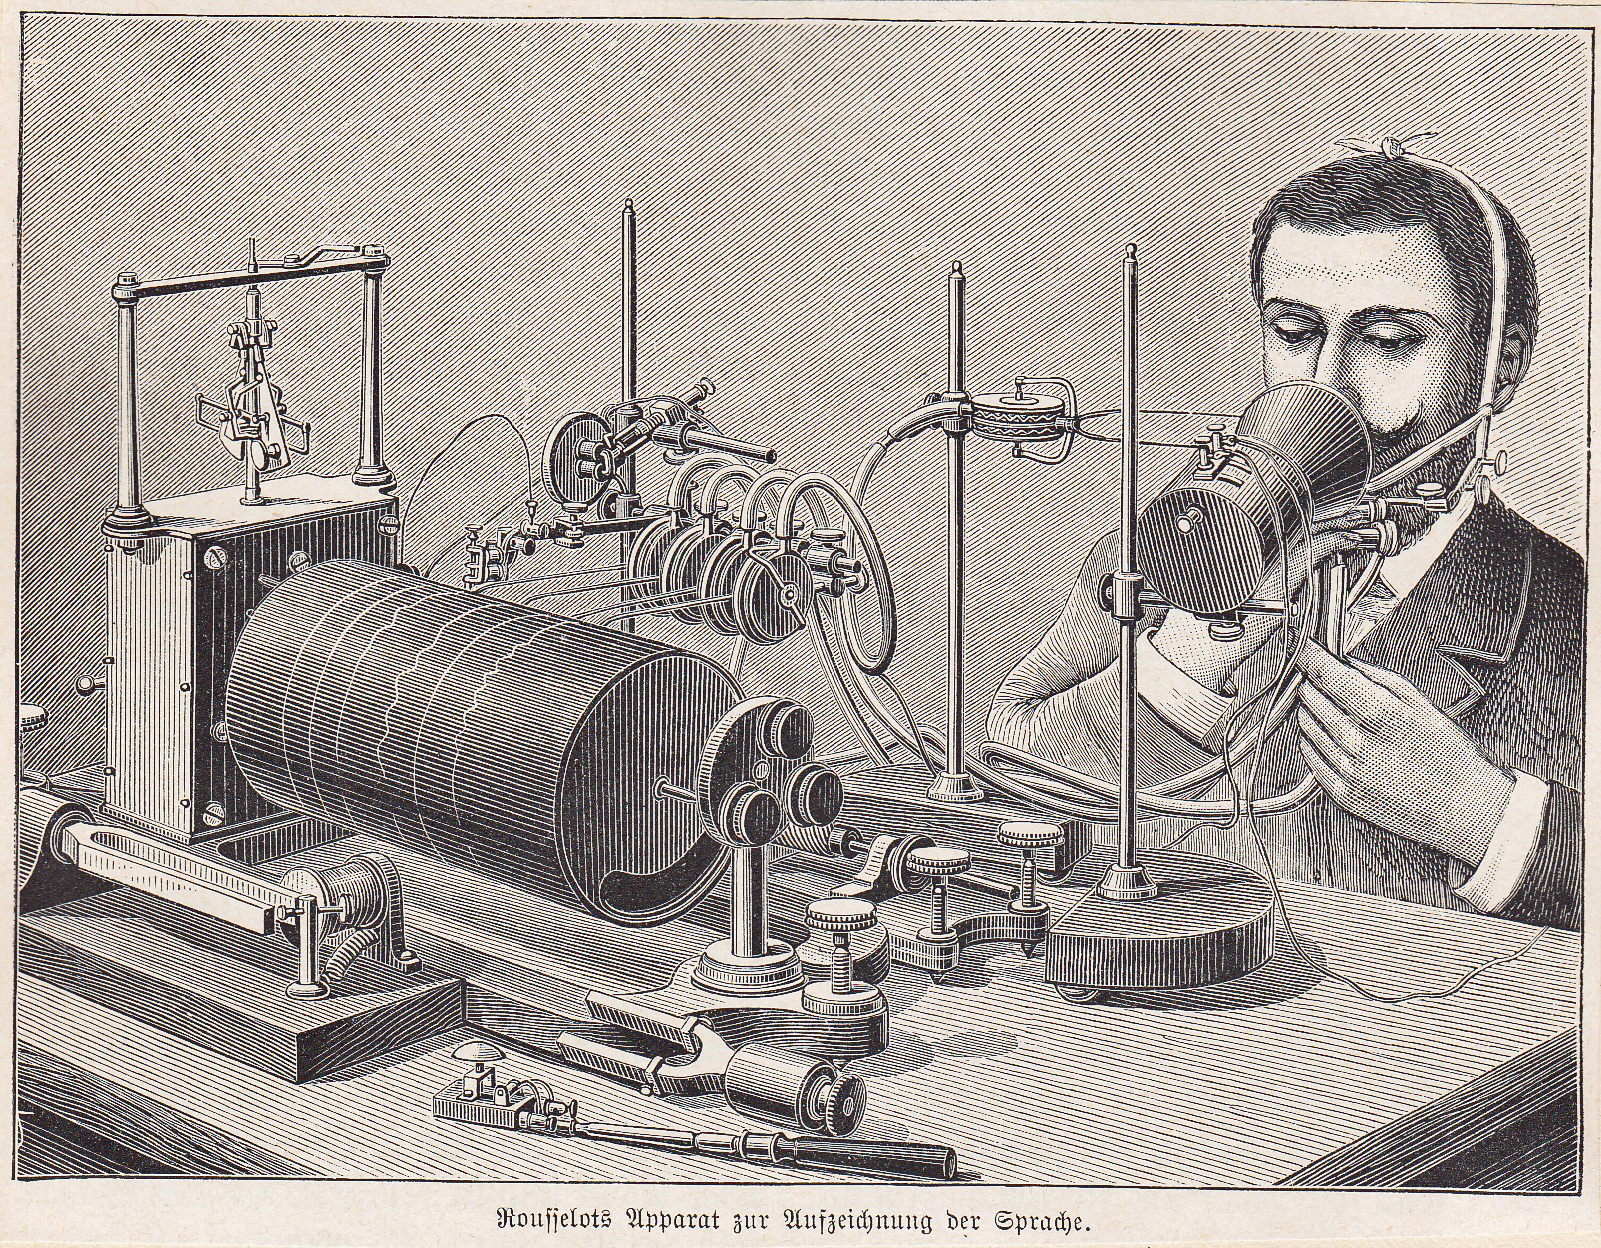
\includegraphics[scale=0.1]{material/04RousselotsApparatzurAufzeichnungderSprache}
		\caption{Rousselots Apparat}
		%{material/04proband}
		%\caption{Proband \citep{Pompino95a}}
		%\label{Zeichen1}
	\end{figure}
	
\end{frame}


%%%%%%%%%%%%%%%%%%%%%%%%%%%%%%%%%%%
%Alternative:

%\begin{frame}{Methodik}

%	\begin{figure}[H]
%		\centering
		
%		\includegraphics[scale=0.07]{material/04Rousselots_Apparat_zu_Aufzeichnung_der_Sprache}
%		\caption{Rousselots Apparat, gemeinfrei, Quelle: Museum für Kommunikation Frankfurt, https://de.wikipedia.org/wiki/Datei:Rousselots_Apparat_zur_Aufzeichnung_der_Sprache.jpg}
		%\label{Zeichen1}
%	\end{figure}
	
%\end{frame}


%%%%%%%%%%%%%%%%%%%%%%%%%%%%%%%%%%%
\begin{frame}
\frametitle{Deskriptive, Symbol-, Instrumental- und Signalphonetik}

	\begin{itemize}
		\item Der geschulte Ohrenphonetiker analysiert und beschreibt das Gehörte
                  (\textbf{deskriptive Phonetik}).

                  Die analysierten Lautkategorien werden anschließend mit symbolischen Mitteln (dem Internationalen Phonetischen Alphabet -- IPA) dargestellt (\textbf{Symbolphonetik}).

		\item Phonetiker nehmen die ablaufenden physikalischen Vorgänge mittels spezieller Mess- oder Registriergeräte während des Sprechaktes als Signale auf (\textbf{Instrumental-} oder \textbf{Signalphonetik}).
	\end{itemize}
	
\end{frame}


%%%%%%%%%%%%%%%%%%%%%%%%%%%%%%%%%%%
\begin{frame}
\frametitle{Methodik: Beispiele}

Messen/Erfassen von
	\begin{itemize}
\item Kiefer-, Lippen- und Zungenbewegungen mithilfe der elektrischen Muskelpotenziale
\item Luftdruckschwankungen, die das akustische Signal darstellen
\item Verlauf des intraoralen Luftdrucks
\item Veränderung der Durchblutung bestimmter Großhirnregionen bei der Verarbeitung von lautsprachlichen Reizen
	\end{itemize}	
\end{frame}


%%%%%%%%%%%%%%%%%%%%%%%%%%%%%%%%%%%
\begin{frame}
\frametitle{Zusammenhang zwischen Experimental- und perzeptiver Phonetik}

	\begin{itemize}
		\item \textbf{Experimentalphonetik} oder \textbf{perzeptive Phonetik} untersucht den
                  Zusammenhang zwischen bestimmten Signalausprägungen und der Wahrnehmung von Versuchspersonen.

                  Damit wird ein Zusammenhang zwischen der Instrumentalphonetik und der deskriptiven Phonetik erzeugt.
	\end{itemize}
	
	\ea	Bei Veränderung von einzelnen akustischen Parametern:\\
	Ab wann nimmt eine Versuchsperson ein \textipa{[ da ]} als \textipa{[ ta ]} wahr?
	\z 
	
\end{frame}


%%%%%%%%%%%%%%%%%%%%%%%%%%%%%%%%%%%
%%%%%%%%%%%%%%%%%%%%%%%%%%%%%%%%%%%
\subsection{Probleme der Phonetik}

%% MyP: Contents
\iftoggle{sectoc}{
	\frame{
		%\begin{multicols}{2}
		\frametitle{~}
		\tableofcontents[currentsubsection,subsubsectionstyle=hide]
		%\end{multicols}
	}
}

%% StM: Contents
\iftoggle{gliederung}{
\outline{

\begin{itemize}

\item Einführung
\item Bereiche der Phonetik
\item  Methodik
\item  \blaubf{Probleme der Phonetik}
\item  IPA-Alphabet
\item Artikulatorische Phonetik
%% Konsonanten
%% Konsonantenklassifikation
%% Vokale
%% Vokalklassifikation
%% Vokalviereck
%% Monophthong, Diphthong, Triphthong
\item Übungen
  
  \end{itemize}
	}
}


%%%%%%%%%%%%%%%%%%%%%%%%%%%%%%%%%%%
\begin{frame}{Probleme der Phonetik: schnelle Übermittlung der Laute}

\begin{itemize}
	\item kurzer Satz (mit 50 Segmenten): ung. 2 Sekunden\\
		\dash bis zu 25 (sprachliche) Segmente pro Sekunde
\medskip
	\item nicht-sprachliche Segmente: ung. 7 bis 9 pro Sekunde
	\item[\ra] Hohe Geschwindigkeit bei der Äußerung eines Satzes macht aus einer sprachlichen Äußerung ein \textbf{Kontinuum}, in dem die Segmentierung der Laute besonders schwer ist.
\end{itemize}


\end{frame}


%%%%%%%%%%%%%%%%%%%%%%%%%%%%%%%%%%%
\begin{frame}
\frametitle{Schallsignal als Kontinuum}

	\begin{figure}[H]
	\centering
	
	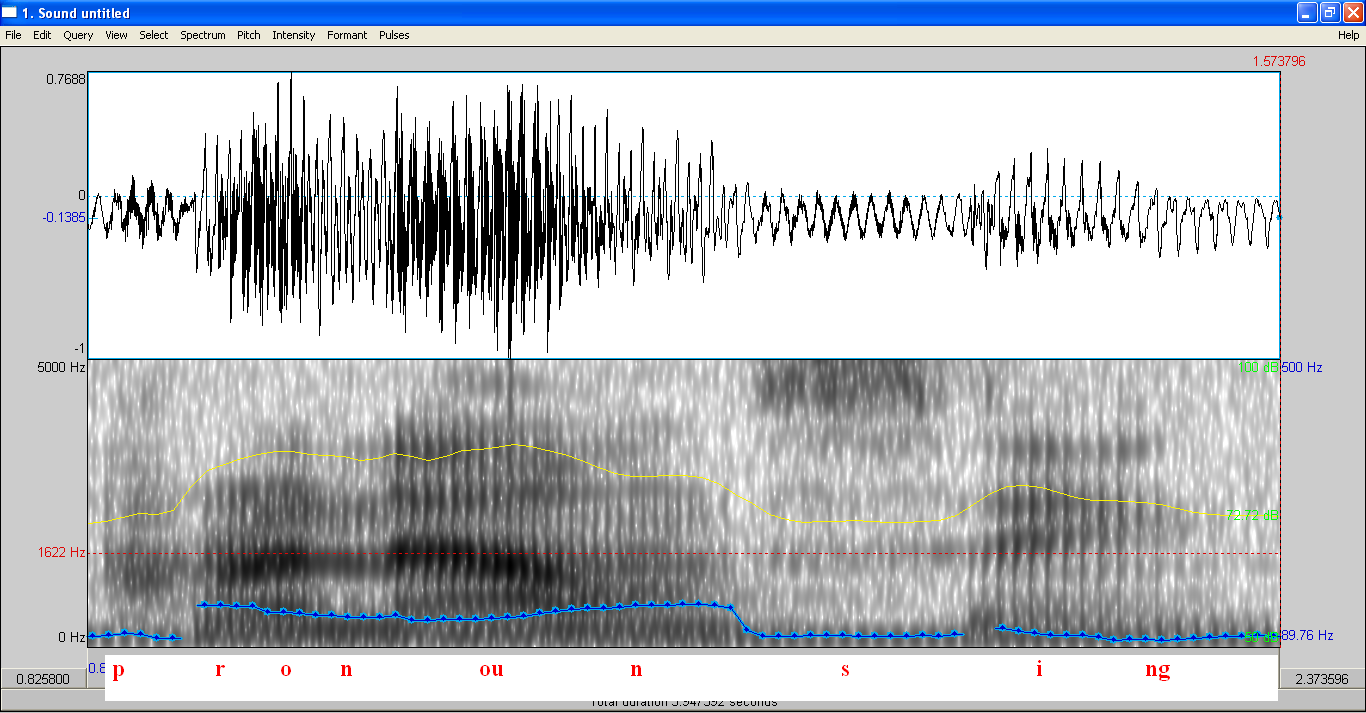
\includegraphics[scale=0.2]{material/04Pronouncing}
	\caption{Spektrogramm des Wortes \emph{pronouncing}}
	%Die alte Version: \includegraphics[scale=0.50]{material/oszillogrammwiese} \caption{\citep{WieseR11a}}
	%\label{Zeichen1}
	\end{figure}

Schallsignal ist ein Kontinuum, eine genaue Segmentierung daher schwierig
	
\end{frame}


%%%%%%%%%%%%%%%%%%%%%%%%%%%%%%%%%%%
\begin{frame}
\frametitlefit{Keine 1-zu-1-Korrespondenz zw.\ Lauten und Verschriftlichung}

\begin{itemize}
			
	\item ein Laut \ras mehrere Buchstaben

	\ea \textipa{[s]} \ras \ab{\textbf{S}maragd}, \ab{gro\textbf{ß}}, \ab{e\textbf{ss}en}
	\z
	
	
	\item eine Buchstabenfolge \ras unterschiedliche Laute

	\ea \ab{ch} \ras \ab{mi\textbf{ch}}, \ab{Bu\textbf{ch}}, \ab{se\textbf{ch}s}, \ab{\textbf{Ch}arme}, \ab{\textbf{Ch}ip}
	\z
	
\end{itemize}

\medskip

\begin{description}
	\item[\textbf{IPA-Alphabet:}] Schriftsystem mit 1-zu-1-Korrespondenz zwischen Lauten und (diakritischen) Zeichen
\end{description}	
		
\end{frame}


%%%%%%%%%%%%%%%%%%%%%%%%%%%%%%%%%%%
%%%%%%%%%%%%%%%%%%%%%%%%%%%%%%%%%%%
\subsection{IPA-Alphabet}

%% MyP: Contents
\iftoggle{sectoc}{
	\frame{
		%\begin{multicols}{2}
		\frametitle{~}
		\tableofcontents[currentsubsection,subsubsectionstyle=hide]
		%\end{multicols}
	}
}

%%StM: Contents
\iftoggle{gliederung}{

\outline{

\begin{itemize}

\item Einführung
\item Bereiche der Phonetik
\item  Methodik
\item  Probleme der Phonetik
\item  \blaubf{IPA-Alphabet}
\item Artikulatorische Phonetik
%% Konsonanten
%% Konsonantenklassifikation
%% Vokale
%% Vokalklassifikation
%% Vokalviereck
%% Monophthong, Diphthong, Triphthong
\item Übungen
  
  \end{itemize}
	}
}


%%%%%%%%%%%%%%%%%%%%%%%%%%%%%%%%%%%
\begin{frame}{IPA-Alphabet}

	\begin{itemize}
		\item IPA: International Phonetic Association \ras IPA-Alphabet
		\item Seit Mitte des 19. Jh. \ras Entwicklung von phonetischen Umschriftsystemen
		\item IPA-Alphabet ist das am weitesten verbreitete System.
		\item Alle Sprachlaute aller natürlichen Sprachen werden eindeutig dargestellt (phonetische Transkription).
\medskip
		\item \textbf{Repräsentation der Phone} \ras in eckigen Klammern \gqq{\textipa{[ ]}}
		\item \textbf{Orthographische Repräsentation} \ras in spitzen Klammern \gqq{$\langle{} \rangle{}$}
\medskip
		\item {Webseite der IPA}: \url{http://internationalphoneticassociation.org}
		\item {Laute zum Testen}: \url{http://www.ipachart.com/}
	\end{itemize}
	
\end{frame}


%%%%%%%%%%%%%%%%%%%%%%%%%%%%%%%%%%%
%\begin{frame}
%\frametitle{IPA-Alphabet}
%
%	\begin{figure}[H]
%		\centering
%		
%		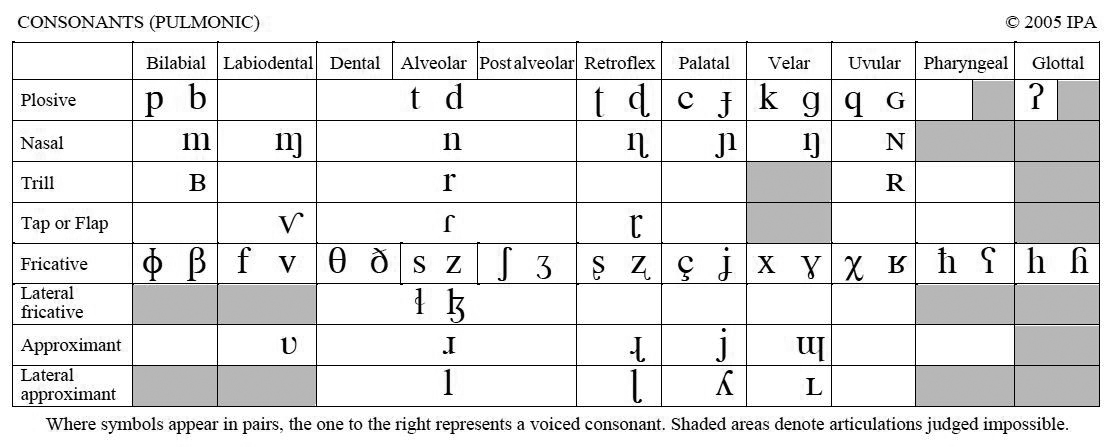
\includegraphics[scale=0.35]{material/04ipaconsonantpulmonic}
%		\caption{Konsonanten (Pulmonal)}
%		%\label{Zeichen1}
%	\end{figure}	
%	
%\end{frame}


%%%%%%%%%%%%%%%%%%%%%%%%%%%%%%%%%%%
\begin{frame}
\frametitle{Pulmonale Konsonanten im IPA-Alphabet}

\begin{table}
\centering
\begin{adjustbox}{max width=\textwidth}
\begin{tabular}{|p{0.1\textwidth}|c|c|c|c|c|c|c|c|c|c|c|c|c|}
\hline
& \tiny{Bilabial} & \tiny{Labiodental} & \tiny{Dental} & \tiny{Alveolar} & \tiny{Postalveolar} & \tiny{Retroflex} & \tiny{Palatal} & \tiny{Velar} & \tiny{Uvular} & \multicolumn{2}{|c|}{\tiny{Pharyngal}} & \multicolumn{2}{|c|}{\tiny{Glottal}} \\
\hline
\tiny{Plosive} & \textipa{p b} & & \multicolumn{3}{|c|}{\textipa{t d}} & \textipa{\:d \:t} & \textipa{c \textbardotlessj} & \textipa{k g} & \textipa{q \textscg} &  & \cellcolor{lightgray} & \textipa{P} & \cellcolor{lightgray} \\
\hline
\tiny{Nasale} & \textipa{m} & \textipa{\textltailm} & \multicolumn{3}{|c|}{\textipa{n}} & \textipa{\textrtailn} & \textipa{\textltailn} & \textipa{\ng} & \textipa{\textscn} & \multicolumn{2}{|c|}{\cellcolor{lightgray}} & \multicolumn{2}{|c|}{\cellcolor{lightgray}} \\
\hline
\tiny{Vibranten} & \textipa{\textscb} & & \multicolumn{3}{|c|}{\textipa{r}} & & & \cellcolor{lightgray} & \textipa{\textscr} & \multicolumn{2}{|c|}{} & \multicolumn{2}{|c|}{\cellcolor{lightgray}} \\
\hline
\tiny{Taps/ Flaps} & & &  \multicolumn{3}{|c|}{\textipa{\textfishhookr}} &  \textipa{\textrtailr} & & \cellcolor{lightgray} & & \multicolumn{2}{|c|}{} & \multicolumn{2}{|c|}{\cellcolor{lightgray}} \\
\hline
\tiny{Frikative} & \textipa{\textphi \textbeta} & \textipa{f v} & \textipa{\texttheta \dh} & \textipa{s z} & \textipa{S Z} & \textipa{\:s \:z} & \textipa{\c{c} J} & \textipa{x G} & \textipa{X \textinvscr} & \multicolumn{2}{|c|}{\textipa{\textcrh \textrevglotstop}} & \multicolumn{2}{|c|}{\textipa{h \texthth}} \\
\hline
\tiny{Laterale Frikative} & \cellcolor{lightgray} & \cellcolor{lightgray} & \multicolumn{3}{|c|}{\textipa{\textbeltl \textlyoghlig}} & & & & &  \multicolumn{2}{|c|}{\cellcolor{lightgray}} & \multicolumn{2}{|c|}{\cellcolor{lightgray}} \\
\hline
\tiny{Approximanten} & & \textipa{\textscriptv} & \multicolumn{3}{|c|}{\textipa{\textturnr}} & \textipa{\:R} & \textipa{j} & \textipa{\textturnmrleg} & & \multicolumn{2}{|c|}{} & \multicolumn{2}{|c|}{\cellcolor{lightgray}} \\
\hline
\tiny{Laterale Approximanten} & \cellcolor{lightgray} & \cellcolor{lightgray} & \multicolumn{3}{|c|}{\textipa{l}} & \textipa{\:l} & \textipa{\textturny} & \textipa{\textscl} & & \multicolumn{2}{|c|}{\cellcolor{lightgray}} & \multicolumn{2}{|c|}{\cellcolor{lightgray}} \\
\hline
\end{tabular}
\end{adjustbox}
%\caption{Pulmonische Konsonanten, IPA. Bei Paaren ist der rechte Konsonant stimmhaft. Graue Flächen gelten als artikulatorisch unmöglich.
	 %https://www.internationalphoneticassociation.org/sites/default/files/pulmonic.gif Stand: 09.12.16
% } 
\end{table}

\begin{itemize}
\item Bei Paaren ist der rechte Konsonant stimmhaft.
\item Graue Flächen gelten als artikulatorisch unmöglich.
\item Achtung: Affrikaten sind hier nicht verzeichnet!
\end{itemize}
  
\end{frame}


%%%%%%%%%%%%%%%%%%%%%%%%%%%%%%%%%%%
\begin{frame}
\frametitle{Nichtpulmonale Konsonanten im IPA-Alphabet}

\begin{table}
	\centering
	\begin{adjustbox}{max width=\textwidth}
		\begin{tabular}{|c c | c c | c c|}
			\hline
			\multicolumn{2}{|c|}{Clicks} & \multicolumn{2}{|c|}{Voiced implosives} & \multicolumn{2}{|c|}{Ejectives} \\
			\hline
			\textipa{\!o} & \tiny{Bilabial} & \textipa{\!b} & \tiny{Bilabial} &  \textipa{'} & \\
			\textipa{\textpipe} & \tiny{Dental} & \textipa{\!d} & \tiny{Dental/alveolar} & \textipa{p'} & \tiny{Bilabial} \\
			\textipa{!} & \tiny{(Post)alveolar} & \textipa{\!j} & \tiny{Palatal} & \textipa{t'} & \tiny{Dental/alveolar} \\
			\textipa{\textdoublebarpipe} & \tiny{Palatoalveolar} & \textipa{\!g} & \tiny{Velar} & \textipa{k'} & \tiny{Velar} \\
			\textipa{\textdoublepipe} & \tiny{Alveolar lateral} & \textipa{\!G} & \tiny{Uvular} & \textipa{s'} & \tiny{Alveolar frikativ} \\
			\hline
		\end{tabular}
	\end{adjustbox}
%	\caption{Nichtpulmonale Konsonanten, IPA.
		%https://www.internationalphoneticassociation.org/sites/default/files/pulmonic.gif Stand: 09.12.16
%	} 
\end{table}

%	\begin{figure}[H]
%		\centering
%		
%		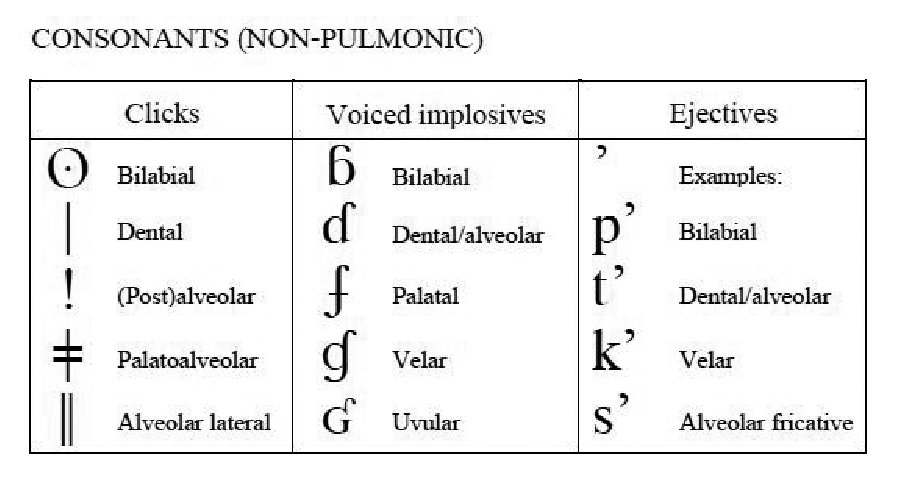
\includegraphics[scale=0.45]{material/04ipaconsonantnonpulmonic}
%		\caption{Konsonanten (Nicht Pulmonal)}
%		%\label{Zeichen1}
%	\end{figure}
	
	\begin{itemize}
		\item \textbf{VIDEO:} \href{run:material/04namaclicks.mp4}{!Nama Clicks}
	\end{itemize}
			
\end{frame}


%%%%%%%%%%%%%%%%%%%%%%%%%%%%%%%%%%%
\begin{frame}
\frametitle{Vokale im IPA-Alphabet: das Vokalviereck}

%	\begin{figure}[H]
%		\centering
%		
%		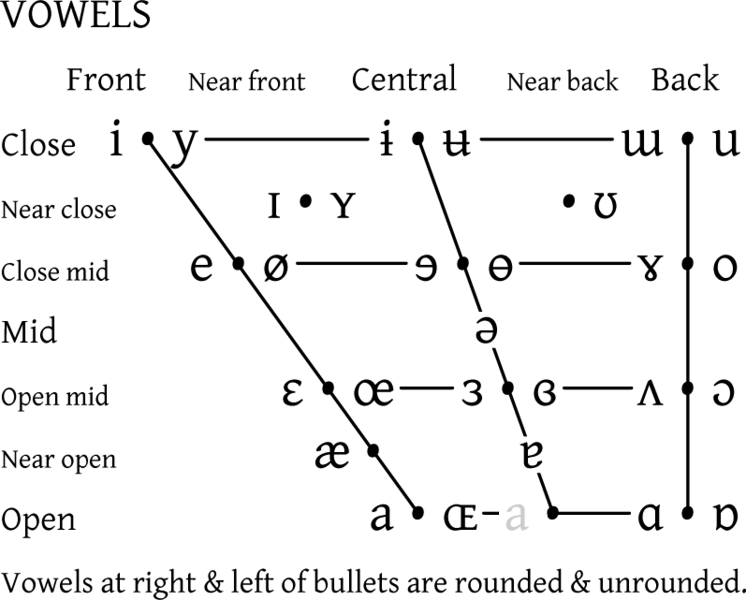
\includegraphics[scale=0.27]{material/04ipavowelwikicommons}
%		\caption{Vokale}
%		%old picture
%		%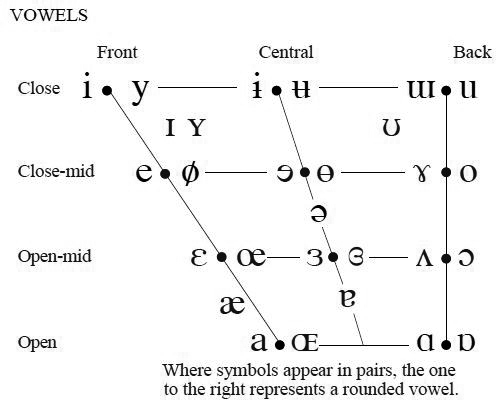
\includegraphics[scale=0.45]{material/04ipavowel}
%		%\caption{Vokale}
%		%\label{Zeichen1}
%	\end{figure}


\centerline{
	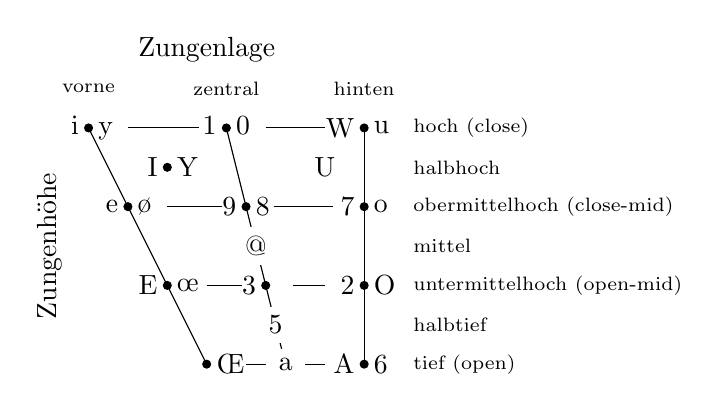
\begin{tikzpicture}
	\draw[fill] (0,0) circle [radius=0.05];
	\draw[fill] (-0.5,1) circle [radius=0.05];
	\draw[fill] (-1,2) circle [radius=0.05];
	\draw[fill] (-1.5,3) circle [radius=0.05];
	\draw[black] (0.5,0)--(0.75,0);
	\draw[black] (1.25,0)--(1.5,0);
	\draw[fill] (2,0) circle [radius=0.05];
	\draw[fill] (2,1) circle [radius=0.05];
	\draw[fill] (2,2) circle [radius=0.05];
	\draw[fill] (2,3) circle [radius=0.05];
	\draw[fill] (0.25,3) circle [radius=0.05];
	\draw[black] (0.25,3)--(1,0);
	\draw[black] (-0.1,3)--(-1,3);
	\draw[black] (0.75,3)--(1.5,3);
	\draw[fill] (0.5,2) circle [radius=0.05];
	\draw[fill] (0.75,1) circle [radius=0.05];
	\node[right] at (0.25,3){\strut \textipa{0}};
	\node[left] at (0.25,3){\strut \textipa{1}};
	\node at (0,4){Zungenlage};
	\node [rotate=90] at (-2,1.5){Zungenhöhe};
	\node at (-1.5,3.5){{\scriptsize vorne}};
	\node at (0.25,3.5){\scriptsize zentral};
	\node at (2,3.5){{\scriptsize hinten}};
	\node[right] at (2.5,3){\scriptsize hoch (close)};
	\node[right] at (2.5,2.5){\scriptsize halbhoch};
	\node[right] at (2.5,2){\scriptsize obermittelhoch (close-mid)};
	\node[right] at (2.5,1.5){\scriptsize mittel};
	\node[right] at (2.5,1){\scriptsize untermittelhoch (open-mid)};
	\node[right] at (2.5,0.5){\scriptsize halbtief};
	\node[right] at (2.5,0){\scriptsize tief (open)};
	\node[left] at (2,3){\textipa{W}};
	\node[right] at (2,3){\textipa{u}};
	\node at (1.5,2.5){\textipa{U}};
	\node[left] at (2,2){\textipa{7}};
	\node[right] at (2,2){\textipa{o}};
	\node[left] at (2,1){\textipa{2}};
	\node[right] at (2,1){\textipa{O}};
	\node[right] at (2,0){\textipa{6}};
	\node[left] at (2,0){\textipa{A}};
	\draw[black] (2,0)--(2,3);
	\node[left] at (0.5,2){\textipa{9}};
	\node[right] at (0.5,2){\textipa{8}};
	\node[rectangle,fill=white] at (0.625,1.5){\textipa{@}};
	\node[left] at (0.75,1){\textipa{3}};
	\node[right] at (0.75,1){\textipa{\textcloserevepsilon}};
	\node[rectangle,fill=white] at (0.875,0.5){\textipa{5}};
	\node[rectangle,fill=white] at (1,0){\textipa{a}};
	\node[right] at (-1.5,3){\strut \textipa{y}};
	\node[left] at (-1.5,3){\strut \textipa{i}};
	\node[left] at (-0.5,2.5){\textipa{I}};
	\node[right] at (-0.5,2.5){\textipa{Y}};
	\draw[fill] (-0.5,2.5) circle [radius=0.05];
	\node[right] at (-1,2){\textipa{\o}};
	\node[left] at (-1,2){\textipa{e}};
	\node[right] at (-0.5,1){\textipa{\oe}};
	\node[left] at (-0.5,1){\textipa{E}};
	\node[right] at (0,0){\textipa{\OE}};
	\draw[black] (0,0)--(-1.5,3);
	\draw[black] (-0.5,2)--(0.2,2);
	\draw[black] (0.85,2)--(1.6,2);
	\draw[black] (0,1)--(0.45,1);
	\draw[black] (1.1,1)--(1.5,1);
	\end{tikzpicture}
}
        
        Vokale links des Punktes sind ungerundet,\\
        die rechts sind gerundet.

%=======
%	\begin{figure}[H]
%		\centering
%		
%		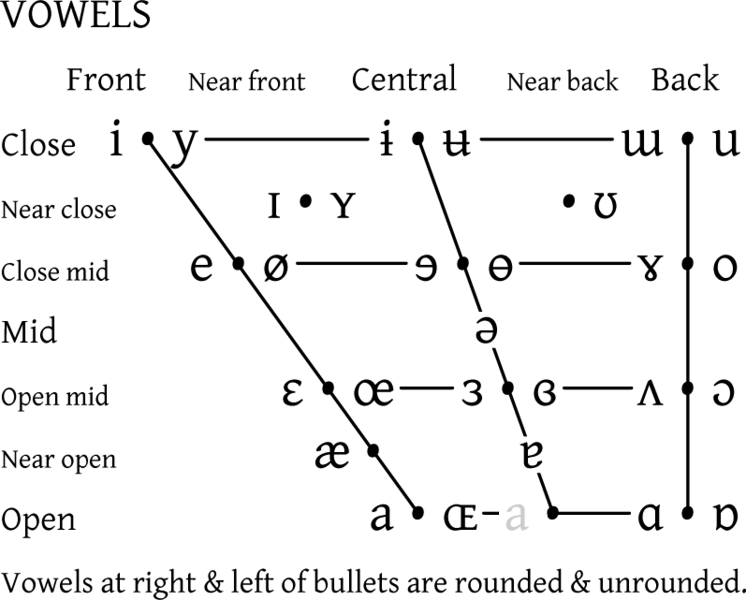
\includegraphics[scale=0.27]{material/04ipavowelwikicommons}
%%		\caption{Vokale}
%		%old picture
%		%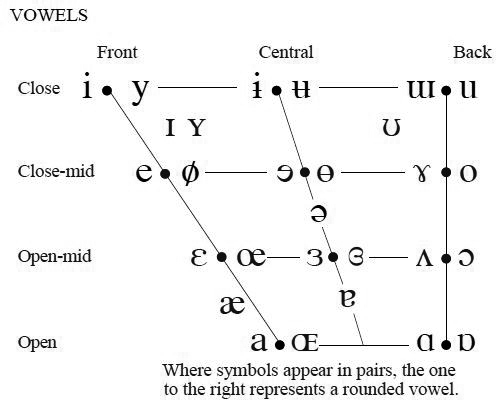
\includegraphics[scale=0.45]{material/04ipavowel}
%		%\caption{Vokale}
%		%\label{Zeichen1}
%	\end{figure}
	
\end{frame}


%%%%%%%%%%%%%%%%%%%%%%%%%%%%%%%%%%%
\begin{frame}
\frametitle{Vokale im Deutschen}

\noindent
\begin{minipage}{.55\textwidth}
	\centerline{
	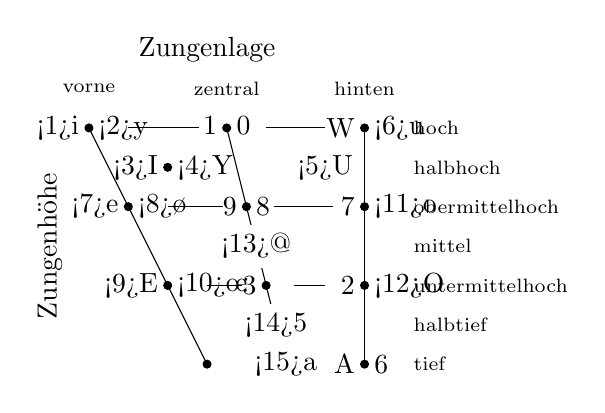
\begin{tikzpicture}
	\draw[fill] (0,0) circle [radius=0.05];
	\draw[fill] (-0.5,1) circle [radius=0.05];
	\draw[fill] (-1,2) circle [radius=0.05];
	\draw[fill] (-1.5,3) circle [radius=0.05];
	\draw[black] (0.5,0)--(0.75,0);
	\draw[black] (1.25,0)--(1.5,0);
	\draw[fill] (2,0) circle [radius=0.05];
	\draw[fill] (2,1) circle [radius=0.05];
	\draw[fill] (2,2) circle [radius=0.05];
	\draw[fill] (2,3) circle [radius=0.05];
	\draw[fill] (0.25,3) circle [radius=0.05];
	\draw[black] (0.25,3)--(1,0);
	\draw[black] (-0.1,3)--(-1,3);
	\draw[black] (0.75,3)--(1.5,3);
	\draw[fill] (0.5,2) circle [radius=0.05];
	\draw[fill] (0.75,1) circle [radius=0.05];
	\node[right] at (0.25,3){\strut \textipa{0}};
	\node[left] at (0.25,3){\strut \textipa{1}};
	\node at (0,4){Zungenlage};
	\node [rotate=90] at (-2,1.5){Zungenhöhe};
	\node at (-1.5,3.5){{\scriptsize vorne}};
	\node at (0.25,3.5){\scriptsize zentral};
	\node at (2,3.5){{\scriptsize hinten}};
	\node[right] at (2.5,3){\scriptsize hoch};
	\node[right] at (2.5,2.5){\scriptsize halbhoch};
	\node[right] at (2.5,2){\scriptsize obermittelhoch};
	\node[right] at (2.5,1.5){\scriptsize mittel};
	\node[right] at (2.5,1){\scriptsize untermittelhoch};
	\node[right] at (2.5,0.5){\scriptsize halbtief};
	\node[right] at (2.5,0){\scriptsize tief};
	\node[left] at (2,3){\textipa{W}};
	\node[right] at (2,3){\rotul{\gruen<6>{\textipa{u}}}};
	\node at (1.5,2.5){\rotul{\gruen<5>{\textipa{U}}}};
	\node[left] at (2,2){\textipa{7}};
	\node[right] at (2,2){\rotul{\gruen<11>{\textipa{o}}}};
	\node[left] at (2,1){\textipa{2}};
	\node[right] at (2,1){\rotul{\gruen<12>{\textipa{O}}}};
	\node[right] at (2,0){\textipa{6}};
	\node[left] at (2,0){\textipa{A}};
	\draw[black] (2,0)--(2,3);
	\node[left] at (0.5,2){\textipa{9}};
	\node[right] at (0.5,2){\textipa{8}};
	\node[rectangle,fill=white] at (0.625,1.5){\rotul{\gruen<13>{\textipa{@}}}};
	\node[left] at (0.75,1){\textipa{3}};
	\node[right] at (0.75,1){\textipa{\textcloserevepsilon}};
	\node[rectangle,fill=white] at (0.875,0.5){\rotul{\gruen<14>{\textipa{5}}}};
	\node[rectangle,fill=white] at (1,0){\rotul{\gruen<15>{\textipa{a}}}};
	\node[right] at (-1.5,3){\rotul{\gruen<2>{\strut \textipa{y}}}};
	\node[left] at (-1.5,3){\rotul{\gruen<1>{\strut \textipa{i}}}};
	\node[left] at (-0.5,2.5){\rotul{\gruen<3>{\textipa{I}}}};
	\node[right] at (-0.5,2.5){\rotul{\gruen<4>{\textipa{Y}}}};
	\draw[fill] (-0.5,2.5) circle [radius=0.05];
	\node[right] at (-1,2){\rotul{\gruen<8>{\textipa{\o}}}};
	\node[left] at (-1,2){\rotul{\gruen<7>{\textipa{e}}}};
	\node[right] at (-0.5,1){\rotul{\gruen<10>{\textipa{\oe}}}};
	\node[left] at (-0.5,1){\rotul{\gruen<9>{\textipa{E}}}};
	\node[right] at (0,0){\textipa{\textscoelig }};
	\draw[black] (0,0)--(-1.5,3);
	\draw[black] (-0.5,2)--(0.2,2);
	\draw[black] (0.85,2)--(1.6,2);
	\draw[black] (0,1)--(0.45,1);
	\draw[black] (1.1,1)--(1.5,1);
	\end{tikzpicture}
}

\medskip

Deutsche Vokale sind \alt<handout>{unterstrichen.}{rot.}
\end{minipage}
\hfill
\begin{minipage}{.42\textwidth}
	\begin{itemize}
	\item Liege [\textipa{li:g@}]\pause,  Lüge [\textipa{ly:g@}]\pause
	\item Kiste [\textipa{kIst@}]\pause,  Küste [\textipa{kYst@}]\pause
	\item muss [\textipa{mUs}]\pause,   Mus   [\textipa{mu:s}]\pause
	\item Wege  [\textipa{ve:g@}]\pause,  wöge [\textipa{vø:g@}]\pause
	\item helle [\textipa{hEl@}]\pause,   Hölle [\textipa{hœl@}]\pause
	\item Ofen  [\textipa{o:f@n}]\pause,  offen [\textipa{Of@n}]\pause
	\item geben [\textipa{ge:b@n}]\pause, Lehrer [\textipa{le:K5}]\pause
	\item Lab   [\textipa{la:p}]
	\end{itemize}
\end{minipage}
\end{frame}


%%%%%%%%%%%%%%%%%%%%%%%%%%%%%%%%%%%
\begin{frame}
\frametitle{Suprasegmentalia}

\begin{tabular}{l|p{6cm}|p{3cm}}
\textbf{Zeichen} &	\textbf{Erklärung} & \textbf{Beispiel} \\
\hline
\alertred{\textipa{\textprimstress}} & Hauptbetonung &[\textipa{Pa.po.\textprimstress te:.k@}]\\

\alertred{\textipa{\textsecstress}} & Nebenbetonung & [\textipa{\textprimstress ba:n.ho:fs.\textsecstress plE:.n@}]\\

\alertred{\textipa{:}} & lang & [\textipa{ba:n}] (vs. [\textipa{ban}])\\

\textipa{;} & halblang & \\

\textipa{\u{}} \textipa{\alertred{\textsubarch{ }}} & extra-kurz/unsilbischer Vokal & [\textipa{stu:d\textsubarch{i}@}], [\textipa{stu:d\u{i}@}]\\

\textipa{\textvertline} & untergeordnete Intonationsgruppe &\\

\textipa{\textdoublevertline} &	übergeordnete Intonationsgruppe & \\

\alertred{\textipa{.}} & Silbengrenze & [\textipa{\textprimstress zIl.bEn.\textsecstress gKEn.\t{ts}@}]\\

\alertred{\textipa{\t{}}} & Doppelartikulation & [\textipa{P\t{aU}to}],  [\textipa{nE\t{ts}}] \\

\alertred{\textipa{\.}} & Silbengelenkmarker & \textipa{[kO\.m@]}\\

\alertred{\textipa{\textsyllabic{ }}} & silbische Konsonanten & \textipa{[kUm.p\textsyllabic{l}]}\\
\end{tabular}

\medskip

Die rot markierten Zeichen werden Sie häufiger in diesem und in zukünftigen Seminaren sehen.

\end{frame}


%%%%%%%%%%%%%%%%%%%%%%%%%%%%%%%%%%%
%%%%%%%%%%%%%%%%%%%%%%%%%%%%%%%%%%%
\subsection{Artikulatorische Phonetik}

%% MyP: Contents
\iftoggle{sectoc}{
	\frame{
		%\begin{multicols}{2}
		\frametitle{~}
		\tableofcontents[currentsubsection,subsubsectionstyle=hide]
		%\end{multicols}
	}
}

%% StM: Contents
\iftoggle{gliederung}{
\outline{

\begin{itemize}

\item Einführung
\item Bereiche der Phonetik
\item  Methodik
\item  Probleme der Phonetik
\item  IPA-Alphabet
\item \blaubf{Artikulatorische Phonetik}
\begin{itemize}
\item Konsonanten
\item Konsonantenklassiffikation
\item Vokale
  \item Vokalklassiffikation
\item Vokalviereck
\item Monophthong, Diphthong, Triphthong
    \end{itemize}
\item Übungen
  
  \end{itemize}
	}
}


%%%%%%%%%%%%%%%%%%%%%%%%%%%%%%%%%%%
\begin{frame}{Artikulatorische Phonetik: Initiator, Generator, Modifikator}

Mehrere Körperteile sind für Erzeugung von Schall nötig:
		
\begin{itemize}
	\item \textbf{Initiator}:\\
	die Lunge \ras (Atmung) erzeugt Luftstrom
	
	\item \textbf{Generator}:\\
	der Kehlkopf (Larynx) mit den Stimmbändern \ras\\
	Luftstrom wird in Schwingung versetzt (Phonation)

	\item \textbf{Frequenz}: Häufigkeit, mit der die Stimmlippen schwingen\\
	\medskip
	Frequenz bestimmt die Tonhöhe:
	
	\begin{itemize}
		\item bei Frauen ung. 230 Hz
		\item bei Männern 120 Hz 
		\item bei Säuglingen 400 Hz
	\end{itemize}

\end{itemize}

\textbf{VIDEO:} \href{run:material/04TransNasalEndoscopy.mp4}{Trans-Nasal Endoscopy}


\end{frame}


%%%%%%%%%%%%%%%%%%%%%%%%%%%%%%%%%%%
\begin{frame}{Artikulatorische Phonetik: Initiator, Generator, Modifikator}

Mehrere Körperteile sind für Erzeugung von Schall nötig:

\begin{itemize}
	\item \textbf{Modifikator}: Rachen-, Mund- und Nasenraum mit den verschiedenen Sprechwerkzeugen (Zunge, Lippen, weicher Gaumen)

\medskip
	
	Unterschiedliche Stellung der Artikulationsorgane verändert den Rohschall des Kehlkopfs zu den wohlunterschiedenen Lauten (Artikulation im engeren Sinne).
\end{itemize}
	
\end{frame}


%%%%%%%%%%%%%%%%%%%%%%%%%%%%%%%%%%%
%%%%%%%%%%%%%%%%%%%%%%%%%%%%%%%%%%%
\subsubsection{Konsonanten}
%%% MyP: Contents
%\iftoggle{sectoc}{
%	\frame{
%		%\begin{multicols}{2}
%		\frametitle{~}
%		\tableofcontents[currentsubsubsection]
%		%\end{multicols}
%	}
%}
%%%%%%%%%%%%%%%%%%%%%%%%%%%%%%%%%%%
\begin{frame}{Konsonanten}

	\begin{itemize}
		\item auch genannt: Mitlaute
		
		\item Die Artikulationsorgane bilden eine \textbf{geräuschverursachende Enge} oder einen \textbf{Verschluss} im Ansatzrohr, \dash die Luft wird oberhalb der Stimmritze (Glottis) zwischen den Stimmbändern behindert.
	\end{itemize}
	
\end{frame}


%%%%%%%%%%%%%%%%%%%%%%%%%%%%%%%%%%%
\begin{frame}
\frametitle{Sagittalschnitt}

\begin{minipage}{0.48\textwidth}
	\begin{figure}
	\centering
	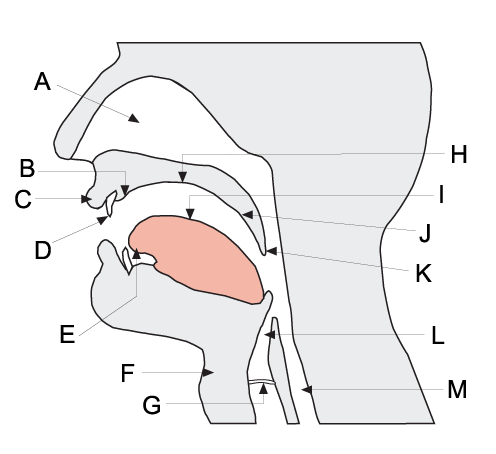
\includegraphics[scale=0.32]{material/04phonoatonomy}
	\caption{Sagittalschnitt}
	\end{figure}
\end{minipage}\hfill
\begin{minipage}{0.4\textwidth}
	A -- Nasenraum\\
	B -- Zahndamm \emph{Alveolen}\\
	C -- (Ober)Lippe \\
	D -- (obere) Zähne\\
	E -- Zungenspitze \emph{Apex}\\
	F -- Kehlkopf \emph{Larynx}\\
	G -- Stimmlippen \emph{Glottis}\\
	H -- harter Gaumen \emph{Palatum}\\
	I -- Zungenrücken \emph{Dorsum}\\
	J -- Gaumensegel \emph{Velum}\\
	K -- Zäpfchen \emph{Uvula}\\
	L -- Luftröhre\\ 
	M -- Speiseröhre
\end{minipage}
	
%	\begin{figure}[H] %%altes Bild%%
%		\centering
%		
%		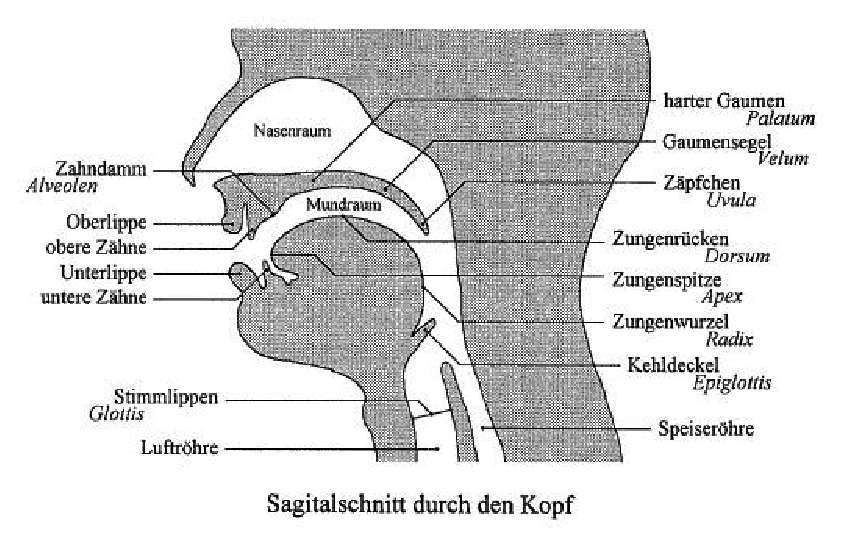
\includegraphics[scale=0.65]{material/04sagitalschnittaltmann}
%		\caption{Sagitalschnitt \citep{Altmann&Co07a}}
%		%\label{Zeichen1}
%	\end{figure}
	
\end{frame}


%%%%%%%%%%%%%%%%%%%%%%%%%%%%%%%%%%%
%%%%%%%%%%%%%%%%%%%%%%%%%%%%%%%%%%%
\subsubsection{Konsonantenklassifikation}
%%% MyP: Contents
%\iftoggle{sectoc}{
%	\frame{
%		%\begin{multicols}{2}
%		\frametitle{~}
%		\tableofcontents[currentsubsubsection]
%		%\end{multicols}
%	}
%}
%%%%%%%%%%%%%%%%%%%%%%%%%%%%%%%%%%%
\begin{frame}{Konsonantenklassifikation: Stimmbeteiligung}

	\begin{itemize}
		\item \textbf{Stimmbeteiligung} (Stimmhaftigkeit): Schwingungszustand der Stimmbänder
		
		\begin{itemize}
			
			\item \textbf{stimmlos} \ras weit auseinander stehende Stimmbänder
			
			\item \textbf{stimmhaft} \ras eng beieinander stehende Stimmbänder
			
			\ea \textipa{[ p ]} vs. \textipa{[ b ]}
			\z

			
			\item \textbf{Aspiration} (Behauchung):\par
				Glottis während der Verschlussphase ist weit gespreizt und schwingt mit.

			\ea \textipa{[ \super h ]}
			\z

                        \textbf{VIDEO:} \href{run:material/02-aspiration.mp4}{Aspiration}
		\end{itemize}

	\end{itemize}
	
\end{frame}


%%%%%%%%%%%%%%%%%%%%%%%%%%%%%%%%%%
\begin{frame}
\frametitle{Übung}
Welche der folgenden Laute sind stimmhaft und welche stimmlos?

\ea \label{ex:02sth}
\textipa{[ d, z, f, v, g, k, P ]}
\z

\end{frame}


%%%%%%%%%%%%%%%%%%%%%%%%%%%%%%%%%%
\iftoggle{ue-loesung}{
	%%%%%%%%%%%%%%%%%%%%%%%%%%%%%%%%%%
%% UE 2 - 02 Phonetik
%%%%%%%%%%%%%%%%%%%%%%%%%%%%%%%%%%

\begin{frame}
\frametitle{Übung -- Lösung}

Welche der folgenden Laute sind stimmhaft und welche stimmlos?

\begin{exe}
\exr{ex:02sth} \textipa{[ d, z, f, v, g, k, P ]}
\end{exe}


\begin{multicols}{2}
	\begin{itemize}
		\item \textbf{stimmhaft:} \textipa{[ d, z, v, g ]}
		
		\ea \textipa{[ d ]}: \ab{Dampf}
		
		\ex \textipa{[ z ]}: \ab{Sinn}
		
		\ex \textipa{[ v ]}: \ab{Wald}
		
		\ex \textipa{[ g ]}: \ab{ganz}
		
		\z 
	\end{itemize}
	
	\columnbreak \pause
	
	\begin{itemize}
		\item \textbf{stimmlos:} \textipa{[ f, k, P ]}
		
		\ea \textipa{[ f ]}: \ab{Fass}
		
		\ex \textipa{[ k ]}: \ab{kalt}
		
		\ex \textipa{[ P ]}: \ab{vereisen}
		
		\z
	\end{itemize}
	
\end{multicols}

\end{frame}


}

%%%%%%%%%%%%%%%%%%%%%%%%%%%%%%%%%%%%
\begin{frame}
\frametitle{Konsonantenklassifikation: Stellung des Gaumensegels}

	\begin{itemize}
		\item \textbf{Stellung des Gaumensegels} (des weichen Gaumens):
		
		\begin{itemize}
			
			\item Nasale Laute (\zB \textipa{ [ m, n ]}) \ras Senkung des weichen Gaumens (Velum)
			
			\item Orale Laute (\zB \textipa{ [ f, a ]}) \ras bei gehobenem Velum
		\end{itemize}
		
		
		\item[] \textbf{LINK:} \href{http://smu-facweb.smu.ca/~s0949176/sammy/}{interaktiver Sagittalschnitt}
	\end{itemize}
	
\end{frame}


%%%%%%%%%%%%%%%%%%%%%%%%%%%%%%%%%%%
\begin{frame}
\frametitle{Konsonantenklassifikation: Artikulationsort (I)}

	\begin{itemize}
	\item \textbf{Artikulationsort} im Vokaltrakt: Ort, an dem die Luft behindert wird
          Unterscheidung nach nicht-beweglichen und beweglichen Artikulatoren

\medskip
		
		\item \textbf{Nicht-bewegliche} Artikulatoren (passiver Artikulator, Artikulationsort im engeren Sinne):
			
		\begin{itemize}
			\item die oberen Zähne \ras \textbf{dental}
			
			\item die Alveolen (Knochendamm hinter den oberen Zähnen) \ras \textbf{alveolar}
			
			\item der harte Gaumen (Palatum) \ras \textbf{palatal}
		\end{itemize}
		
	\end{itemize}
	
\end{frame}


%%%%%%%%%%%%%%%%%%%%%%%%%%%%%%%%%%%
\begin{frame}
\frametitle{Konsonantenklassifikation: Artikulationsort (II)}

\begin{itemize}
	\item \textbf{Bewegliche} Artikulatoren (aktiver Artikulator, Artikulationsorgan):
			
	\begin{itemize}
		
		\item weicher Gaumen (Velum) \ras \textbf{velar}
		
		\item das Zäpfchen (Uvula) \ras \textbf{uvular}
		
		\item Lippen \ras \textbf{labial}
		
		\item Unterkiefer
		
		\item Zunge
	\end{itemize}

\end{itemize}

\end{frame}


%%%%%%%%%%%%%%%%%%%%%%%%%%%%%%%%%%%
\begin{frame}
\frametitle{Konsonantenklassifikation: Artikulationsort (III)}

		\begin{itemize}
			\item Bei der Artikulation mit der \textbf{Zunge} bildet man Untergruppen nach dem \textbf{beteiligten Zungenteil}:
			
			\begin{itemize}
				\item \textbf{koronal}: mit dem vorderen Teil der Zunge
	
				\begin{itemize}
					\item \textbf{apikal}: mit der Zungenspitze
					
					\item \textbf{laminal}: mit dem Zungenblatt (mittlerer Teil der Zunge)				
				\end{itemize}
	
				\ea \textipa{[ t, d, l, n, s, z, S, Z ]}
				\z

\pause

				\item \textbf{dorsal}: mit dem hinteren Teil der Zunge

				\ea \textipa{[ \c{c}, j, g, k, x, N, \textscr, K ]}
				\z

			\end{itemize}

					
		\item[] \textbf{LINK:} \href{http://smu-facweb.smu.ca/~s0949176/sammy/}{Interaktiver Sagittalschnitt}

		\end{itemize}
		
\end{frame}


%%%%%%%%%%%%%%%%%%%%%%%%%%%%%%%%%%%
\begin{frame}
\frametitle{Konsonantenklassifikation: Artikulationsart}

	\begin{block}{Artikulationsart}
	(auch Artikulationsmodus)\\
	Art der Behinderung des Luftstroms durch die Artikulationsorgane
	\end{block}	

\end{frame}


%%%%%%%%%%%%%%%%%%%%%%%%%%%%%%%%%%%
\begin{frame}
\frametitle{Artikulationsart: Plosive}

\begin{itemize}
			\item \textbf{Plosive} (Verschlusslaute, Explosivlaute, stops): totaler oraler Verschluss mit anschließender plötzlicher Lösung des Verschlusses\\
				Das Velum bleibt dabei in angehobener Position,\par
				so dass die Luft durch den Mundraum strömt.

			\ea \textipa{[ p, b, t, d, k, g, P ]}
			\z
			
			Der \textbf{Glottalverschluss} (Knacklaut) \textipa{[ P ]} entsteht durch plötzliches Öffnen der Stimmritze und kommt im Deutschen vor anlautendem Vokal eines Wortes und vor anlautendem Vokal in einer betonten Silbe vor.
		
	\end{itemize}
	
\end{frame}


%%%%%%%%%%%%%%%%%%%%%%%%%%%%%%%%%%%
\begin{frame}
\frametitle{Artikulationsart: Frikative}

		\begin{itemize}
			\item \textbf{Frikative} (Reibelaute, Spiranten): Verengung zweier Sprechorgane,\\
                          Luftstrom strömt durch die Verengung, es entsteht ein Reibegeräusch.

			\ea \textipa{[ f, v, s, z, S, Z, \c{c}, x, h, K ]}
			\z

\pause 
			
			\begin{itemize}
				\item \textbf{Sibilanten} (Zischlaut):\par
					Unterklasse der Frikative mit intensivem, hochfrequentem Geräuschanteil.

				\ea \textipa{[ s, z, S ]}
				\z

		\end{itemize}
		
	\end{itemize}
	
\end{frame}


%%%%%%%%%%%%%%%%%%%%%%%%%%%%%%%%%%%
\begin{frame}
%\frametitle{Konsonantenklassifikation}
\frametitle{Artikulationsart: Affrikaten}

		\begin{itemize}
			\item \textbf{Affrikaten}: Plosive, die in Frikative übergehen, wobei die Verschlussphase und die Frikativphase dieselbe (oder annähernd dieselbe) Artikulationsstelle haben; d.\,h. sie sind \textbf{homorgan}.

			\ea \textipa{[ \texttoptiebar{pf}, \texttoptiebar{ts}, \texttoptiebar{tS}, \texttoptiebar{dZ} ]} %\textipa{ \t{aUI}}
			\z

			\begin{itemize}
				\item Per Definition gehören der plosive und der frikative Laut einer Affrikaten \textbf{zum selben Morphem} (die kleinste bedeutungstragende Einheit). Daraus ergibt sich:

				\ea \textipa{[ \t{ts} ]} in \ab{Blitz} \ras Affrikate
				\z
				
				\ea \textipa{[ ts ]} in \ab{Monats} \ras keine Affrikate
				\z

			\end{itemize}
		
		
		\item Plosive, Frikative und Affrikaten \ras \textbf{Obstruenten}
	\end{itemize}
	
\end{frame}


%%%%%%%%%%%%%%%%%%%%%%%%%%%%%%%%%%%
\begin{frame}
\frametitle{Artikulationsart: Vibranten}

		\begin{itemize}
			\item \textbf{Vibranten} (trills): schnelle Folge oraler Verschlüsse
			\begin{itemize}
				
				\item Artikulationsstellen für Vibranten sehr eingeschränkt: nur bilabial, alveolar oder uvular
				
				\item Der alveolare Vibrant \textipa{[ r ]} (das sog. Zungenspitzen-R) kommt in vielen süddeutschen Varietäten vor.
				
				\item Der uvulare Vibrant \textipa{[ \textscr\ ]} (das gerollte Zäpfchen-R) ist eine häufige Realisierung des Deutschen \ab{r}.
			\end{itemize}
			 
	\end{itemize}
	
\end{frame}


%%%%%%%%%%%%%%%%%%%%%%%%%%%%%%%%%%%
\begin{frame}
\frametitle{Artikulationsart: Approximanten}

		\begin{itemize}
			\item \textbf{Approximanten} (Öffnungslaute): Enge im Ansatzrohr (wie Frikative)\\
			Bei Approximanten gibt es nicht so eine große Nähe zwischen Artikulator und Artikulationsstelle \ras kein Reibegeräusch
			
			 Zwei Unterklassen:
			
			\begin{itemize}
				
				\item \textbf{Laterale}: Verschluss in der Mundhöhlenmitte, Luft entweicht seitlich [~\textipa{l}~]
				
				\item \textbf{Gleitlaute} (zentral): zentrale Verengung, aber weiter als bei Frikativen [~\textipa{w}~].\\
				(Manchmal wird [~\textipa{j}~] auch zu den Gleitlauten gezählt,\\
                                  da die Verengung weiter als bei anderen Frikativen ist. Dies ist jedoch strittig.)
			\end{itemize}
			
		\end{itemize}	

\end{frame}


%%%%%%%%%%%%%%%%%%%%%%%%%%%%%%%%%%%
\begin{frame}
%\frametitle{Konsonantenklassifikation}
\frametitle{Artikulationsart: Nasale}
		\begin{itemize}
			\item \textbf{Nasale}: totaler oraler Verschluss (wie Plosive).\\
				Luft entweicht durch die Nase durch Senken des Velums.
			 
			 \ea \textipa{[ m, n, N ]}
			 \z
		
		\item Vibranten, Approximanten (Laterale und Gleitlaute), Nasale und Vokale (auch die hier nicht behandelten \gqq{geschlagenen Laute} wie das span. \textipa{[~R~]}) gehören zur Gruppe der \textbf{Sonoranten}, da die Luft ungehindert ausströmen kann. Sonoranten sind \textbf{immer} stimmhaft!
		
		\item Die Klasse der l-Laute und r-Laute werden auch zu den sog. \textbf{Liquiden} zusammengefasst (im Dt. \textipa{[ l, r, \textscr ]})
	\end{itemize}

	
\end{frame}


%%%%%%%%%%%%%%%%%%%%%%%%%%%%%%%%%%%
\begin{frame}
	\frametitle{Konsonantenklassifikation: Zusammenfassung I}
	
\begin{figure}
	\centering
	
\scalebox{.85}{
\begin{forest}
	sm edges
	[Konsonanten
		[\textbf{Obstruenten}\\{[}$-$son{]}
			[Frikative\\{[}$+$kont{]}
				[{[}$+$sth{]} [\textipa{v z Z}, no edge] ]
				[{[}$-$sth{]} [\textipa{f s S \c{c}}, no edge] ]
			]
			[Plosive\\{[}$-$kont{]}
				[{[}$+$sth{]} [\textipa{b d g}, no edge] ]
				[{[}$-$sth{]} [\textipa{p t k}, no edge] ]
			]
		]
		[\textbf{Sonoranten}\\{[}$-$son{]}
			[Liquide\\{[}$-$nas{]}
				[Laterale\\{[}$+$lat{]} [\textipa{l}, no edge] ]
				[Vibranten\\{[}$-$lat{]} [\textipa{r  R K}, no edge] ]
			]
			[Nasale\\{[}$+$nas{]} [\textipa{m n N}, no edge] ]
		]
	]
\end{forest}
}

\end{figure}

Zur Gruppe der \textbf{Sonoranten} zählen alle Konsonanten, bei denen die Luft \textbf{ungehindert} ausströmen kann. Sie sind \textbf{immer stimmhaft}.

Obstruenten können stimmhaft oder auch stimmlos sein.
	
\end{frame}


%%%%%%%%%%%%%%%%%%%%%%%%%%%%%%%%%%%
\begin{frame}
	\frametitle{Konsonantenklassifikation: Zusammenfassung II}

	\begin{itemize}
		\item Für die \textbf{Differenzierung der deutschen Konsonanten} sind hauptsächlich 3 Merkmale wichtig:
		
		\begin{itemize}
			
			\item Stimmbeteiligung
			\item Artikulationsort
			\item Artikulationsart
		\end{itemize}
	\end{itemize}

\textbf{LINK}: \href{http://www.ipachart.com/}{Interactive IPA chart}

\end{frame}


%%%%%%%%%%%%%%%%%%%%%%%%%%%%%%%%%%
\begin{frame}

\frametitle{Übung}

\begin{itemize}
	\item[] Beschreiben Sie die Konsonanten in den folgenden Wörtern und geben Sie die entsprechenden phonetischen Symbole an:
	
	\begin{enumerate}
		\item Busch
		\item malen
		\item Maus
		\item Achtung
		\item Genie
		\item zirpen
		\item wichtig
		\item Wald
	\end{enumerate}
	
\end{itemize}
\end{frame}


%%%%%%%%%%%%%%%%%%%%%%%%%%%%%%%%%%%
\iftoggle{ue-loesung}{
	%%%%%%%%%%%%%%%%%%%%%%%%%%%%%%%%%%
%% UE 3 - 02 Phonetik
%%%%%%%%%%%%%%%%%%%%%%%%%%%%%%%%%%

\begin{frame}
\frametitle{Übung -- Lösung}

\begin{table}
\scalebox{.9}{
	\begin{tabular}{llp{9cm}}
		1. Busch & \only<2->{[\textipa{bUS}]} & \only<3->{\textipa{b}: bilabialer, stimmhafter Plosiv; \textipa{S}:~postalveolarer, stimmloser Frikativ} \\
		
		2. malen & \only<4->{[\textipa{\textprimstress ma:l@n}]} & \only<5->{\textipa{m}:~bilabialer, stimmhafter Nasal; \textipa{n}:~alveolarer, stimmhafter Nasal, \textipa{l}:~alveolar, stimmhafter Lateral} \\
		
		3. Maus & \only<6->{[\textipa{m\texttoptiebar{aU}s}]} & \only<7->{\textipa{m}:~s.\,o.; \textipa{s}:~stimmloser, alveolarer Frikativ} \\
		
		4. Achtung & \only<8->{[\textipa{\textprimstress PaXtU\ng}]} & \only<9->{\textipa{P}:~glottaler, stimmloser Plosiv; \textipa{X}:~velarer, stimmloser Frikativ; \textipa{t}:~alveolarer, stimmloser Plosiv \textipa{\ng}: velarer, stimmhafter Nasal} \\

		5. Genie & \only<10->{[\textipa{Ze:\textprimstress ni:}]} & \only<11->{\textipa{Z}: postalveolarer, stimmhafter Frikativ, \textipa{n}:~s.\,o.} \\                
		                                                                                  
		6. zirpen & \only<12->{[\textipa{\texttoptiebar{ts}IKp@n}]} & \only<13->{\textipa{\texttoptiebar{ts}}: alveolare, stimmlose Affrikate; \textipa{K}:~uvularer, stimmhafter Frikativ; \textipa{p}:~bilabialer, stimmloser Plosiv; \textipa{n}: s.\,o.} \\

		7. wichtig & \only<14->{[\textipa{\textprimstress vI\c{c}tI\c{c}}]} & \only<15->{\textipa{v}: labiodentaler, stimmhafter Frikativ; \textipa{\c{c}}: palataler, stimmloser Frikativ \textipa{t}: s.\,o.} \\

		8. Wald & \only<16->{[\textipa{valt}]} & \only<17->{\textipa{v, l, t}: s.\,o.}
\end{tabular}
}
\end{table}

\end{frame}

}
%%%%%%%%%%%%%%%%%%%%%%%%%%%%%%%%%%%

%%%%%%%%%%%%%%%%%%%%%%%%%%%%%%%%%%
%%%%%%%%%%%%%%%%%%%%%%%%%%%%%%%%%%
\subsubsection{Vokale}

%%% MyP: Contents
%\iftoggle{sectoc}{
%	\frame{
%		%\begin{multicols}{2}
%		\frametitle{~}
%		\tableofcontents[currentsubsubsection]
%		%\end{multicols}
%	}
%}
%%%%%%%%%%%%%%%%%%%%%%%%%%%%%%%%%%%
\begin{frame}{Vokale}

	\begin{itemize}
		\item \textbf{Vokale} (Selbstlaute) sind Laute, bei deren Artikulation die Luft ungehindert durch den Mundraum strömen kann (deswegen gehören sie zu den \textbf{Sonoranten}).
		
		\item Vokale sind \idR immer \textbf{stimmhaft}.
		
		\item Es ist umstritten, ob der sog. Schwa-Laut im Dt. \textipa{[ @ ]} stimmhaft
                  ist.\\
                  Auch im Japanischen soll es stimmlose Vokale geben.
	\end{itemize}
	
\end{frame}


%%%%%%%%%%%%%%%%%%%%%%%%%%%%%%%%%%%
%%%%%%%%%%%%%%%%%%%%%%%%%%%%%%%%%%%
\subsubsection{Vokalklassifikation}
%%% MyP: Contents
%\iftoggle{sectoc}{
%	\frame{
%		%\begin{multicols}{2}
%		\frametitle{~}
%		\tableofcontents[currentsubsubsection]
%		%\end{multicols}
%	}
%}
%%%%%%%%%%%%%%%%%%%%%%%%%%%%%%%%%%%

\begin{frame}{Vokalklassifikation I}

	\begin{itemize}
		\item \textbf{Zungenhöhe} (Vokalhöhe): Grad der Zungenhebung in Richtung Gaumen

		\ea hoch: \textipa{[ i: ]}, mittel: \textipa{[ o: ]}, tief: \textipa{[ a: ]} bzw. geschlossen, halboffen, offen
		\z

\pause 

		\item \textbf{Zungenlage} (Vokaltiefe): angehobener Teil der Zunge

		\ea vorne: \textipa{[ i: ]}, zentral: \textipa{[ a: ]}, hinten: \textipa{[ u: ]}
		\z

\pause 

		\item \textbf{Lippenrundung}: Art der Lippenöffnung

		\ea gerundet: \textipa{[ o: ]}, ungerundet: \textipa{[ i: ]}
		\z

		\bigskip
 

 	\item Lesen Sie folgende Wörter mit \textbf{gerundeten} und mit \textbf{gespreizten} Lippen:
	\ea 
	\ea Bühne, rühmen, Dünen, Stiele, Trieb, Möhre, Herd, Hefe, kennen

\pause 	

	\ex  Biene, Riemen, dienen, Stühle, trüb, Meere, hört, Höfe, können
	\z  
	\z 
 
\end{itemize}

\end{frame}


%%%%%%%%%%%%%%%%%%%%%%%%%%%%%%%%%%%
\begin{frame}
\frametitle{Vokalklassifikation II}

\begin{itemize}
	\item Gespanntheit:

\begin{description}
	\item[\textbf{Definition 1}] \textipa{[ i:, y:, u:, o: ]} mit \textbf{mehr Muskelspannung} als \textipa{[ I, Y, U, O ]} 
	
	(von der experimentellen Phonetik weder bestätigt noch widerlegt)
	
	\item[\textbf{Definition 2}] \textipa{[ i:, y:, u:, o: ]}  mit \textbf{vorverlagerter Zungenwurzel}


\begin{multicols}{2}

\textbf{gespannt:}
	\ea \textipa{[ i: ]}: \ab{Liege}
	
	\ex \textipa{[ y: ]}: \ab{Lüge}
	
	\ex \textipa{[ u: ]}: \ab{Mus}
	
	\ex \textipa{[ o: ]}: \ab{Ofen}
	
	\z 
	
\columnbreak
	
\textbf{ungespannt:}
	\ea \textipa{[ I ]}: \ab{Kiste}
	
	\ex \textipa{[ Y ]}: \ab{Küste}
	
	\ex \textipa{[ U ]}: \ab{muss}
	
	\ex \textipa{[ O ]}: \ab{offen}
	
	\z
	
\end{multicols}

\end{description}
\end{itemize}
			
\end{frame}		

%%%%%%%%%%%%%%%%%%%%%%%%%%%%%%%%%%%			
			
\begin{frame}
\frametitle{Anmerkungen zur Gespanntheit}
		\begin{itemize}	
			\item i.\,d.\,R. alle tiefen Vokale \ras ungespannt (strittig!)
			\item langer tiefer Vokal \textipa{[ a: ]} \ras gespannt(?)
%		\end{itemize}

	      \item im Deutschen: Korrelation der Gespanntheit mit der Länge

		\ea \textipa{[ m i: t @ ]} vs. \textipa{[ m I t @ ]}
		\z

		\item in Lehnwörtern auch kurze gespannte Vokale

		\ea \textipa{[ P i . d e: ]}
		\z
		
	\end{itemize}
	
\end{frame}


%%%%%%%%%%%%%%%%%%%%%%%%%%%%%%%%%%%
\begin{frame}
\frametitle{Vokalklassifikation III}

	\begin{itemize}
	
		
%\vspace{1em}
		
		\item \textbf{Stellung des Gaumensegels}:
		
		\begin{itemize}
			\item oral
			\item nasal
			
			\item Nasalvokale kommen im Dt. nur in Lehnwörtern vor.

			\eal
			\ex \textipa{[ \~a ]} in \ab{Restaur\textbf{ant}}
			\ex \textipa{[ \~E ]} in \ab{T\textbf{eint}}
			\ex \textipa{[ \~o ]} in \ab{Balk\textbf{on}}
			\ex \textipa{[ \~\oe\ ]} in \ab{in Parf\textbf{um}}
			\zl
		
		\end{itemize}
		
	\end{itemize}
	
\end{frame}


%%%%%%%%%%%%%%%%%%%%%%%%%%%%%%%%%%%
\begin{frame}
\frametitle{Vokalklassifikation: Überblick}

	\begin{itemize}
		\item Für die \textbf{Differenzierung der deutschen nativen Vokale} sind hauptsächlich vier Merkmale wichtig:
		
		\begin{itemize}
			
			\item Zungenhöhe
			
			\item Zungenlage
			
			\item Lippenrundung
			
			\item Gespanntheit (bzw. Länge)
		\end{itemize}
		
	\end{itemize}

\textbf{LINK}: \href{http://www.ipachart.com/}{Interactive IPA chart}
	
\end{frame}


%%%%%%%%%%%%%%%%%%%%%%%%%%%%%%%%%%%
%%%%%%%%%%%%%%%%%%%%%%%%%%%%%%%%%%%
\subsubsection{Vokalviereck}
%%% MyP: Contents
%\iftoggle{sectoc}{
%	\frame{
%		%\begin{multicols}{2}
%		\frametitle{~}
%		\tableofcontents[currentsubsubsection]
%		%\end{multicols}
%	}
%}
%%%%%%%%%%%%%%%%%%%%%%%%%%%%%%%%%%%

\begin{frame}{Vokalviereck}

	\begin{itemize}
		\item Vokale wurden 1920 von Daniel Jones im sog. Vokalviereck angeordnet.
		\item Vokalviereck stellt eine stilisierte Version des Vokalraums dar.
	\end{itemize}

\begin{figure}
	\centering
%\scalebox{.8}{	
	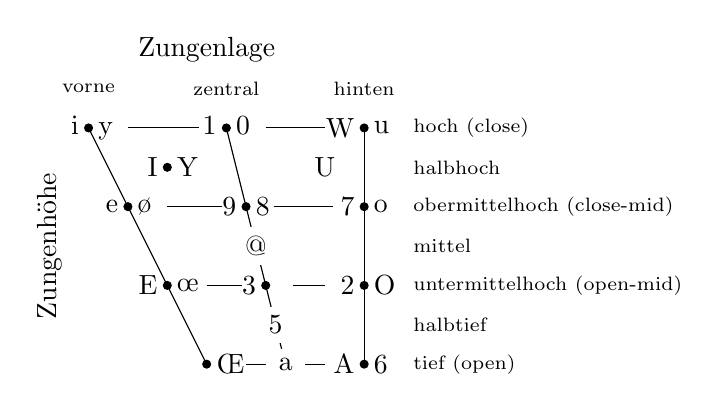
\begin{tikzpicture}
	\draw[fill] (0,0) circle [radius=0.05];
	\draw[fill] (-0.5,1) circle [radius=0.05];
	\draw[fill] (-1,2) circle [radius=0.05];
	\draw[fill] (-1.5,3) circle [radius=0.05];
	\draw[black] (0.5,0)--(0.75,0);
	\draw[black] (1.25,0)--(1.5,0);
	\draw[fill] (2,0) circle [radius=0.05];
	\draw[fill] (2,1) circle [radius=0.05];
	\draw[fill] (2,2) circle [radius=0.05];
	\draw[fill] (2,3) circle [radius=0.05];
	\draw[fill] (0.25,3) circle [radius=0.05];
	\draw[black] (0.25,3)--(1,0);
	\draw[black] (-0.1,3)--(-1,3);
	\draw[black] (0.75,3)--(1.5,3);
	\draw[fill] (0.5,2) circle [radius=0.05];
	\draw[fill] (0.75,1) circle [radius=0.05];
	\node[right] at (0.25,3){\strut \textipa{0}};
	\node[left] at (0.25,3){\strut \textipa{1}};
	\node at (0,4){Zungenlage};
	\node [rotate=90] at (-2,1.5){Zungenhöhe};
	\node at (-1.5,3.5){{\scriptsize vorne}};
	\node at (0.25,3.5){\scriptsize zentral};
	\node at (2,3.5){{\scriptsize hinten}};
	\node[right] at (2.5,3){\scriptsize hoch (close)};
	\node[right] at (2.5,2.5){\scriptsize halbhoch};
	\node[right] at (2.5,2){\scriptsize obermittelhoch (close-mid)};
	\node[right] at (2.5,1.5){\scriptsize mittel};
	\node[right] at (2.5,1){\scriptsize untermittelhoch (open-mid)};
	\node[right] at (2.5,0.5){\scriptsize halbtief};
	\node[right] at (2.5,0){\scriptsize tief (open)};
	\node[left] at (2,3){\textipa{W}};
	\node[right] at (2,3){\textipa{u}};
	\node at (1.5,2.5){\textipa{U}};
	\node[left] at (2,2){\textipa{7}};
	\node[right] at (2,2){\textipa{o}};
	\node[left] at (2,1){\textipa{2}};
	\node[right] at (2,1){\textipa{O}};
	\node[right] at (2,0){\textipa{6}};
	\node[left] at (2,0){\textipa{A}};
	\draw[black] (2,0)--(2,3);
	\node[left] at (0.5,2){\textipa{9}};
	\node[right] at (0.5,2){\textipa{8}};
	\node[rectangle,fill=white] at (0.625,1.5){\textipa{@}};
	\node[left] at (0.75,1){\textipa{3}};
	\node[right] at (0.75,1){\textipa{\textcloserevepsilon}};
	\node[rectangle,fill=white] at (0.875,0.5){\textipa{5}};
	\node[rectangle,fill=white] at (1,0){\textipa{a}};
	\node[right] at (-1.5,3){\strut \textipa{y}};
	\node[left] at (-1.5,3){\strut \textipa{i}};
	\node[left] at (-0.5,2.5){\textipa{I}};
	\node[right] at (-0.5,2.5){\textipa{Y}};
	\draw[fill] (-0.5,2.5) circle [radius=0.05];
	\node[right] at (-1,2){\textipa{\o}};
	\node[left] at (-1,2){\textipa{e}};
	\node[right] at (-0.5,1){\textipa{\oe}};
	\node[left] at (-0.5,1){\textipa{E}};
	\node[right] at (0,0){\textipa{\OE}};
	\draw[black] (0,0)--(-1.5,3);
	\draw[black] (-0.5,2)--(0.2,2);
	\draw[black] (0.85,2)--(1.6,2);
	\draw[black] (0,1)--(0.45,1);
	\draw[black] (1.1,1)--(1.5,1);
	\end{tikzpicture}
%}
	\caption{Vokalviereck}
\end{figure}	
	
\end{frame}


%%%%%%%%%%%%%%%%%%%%%%%%%%%%%%%%%%%
%%%%%%%%%%%%%%%%%%%%%%%%%%%%%%%%%%%
\subsubsection{Monophthong, Diphthong, Triphthong}
%%% MyP: Contents
%\iftoggle{sectoc}{
%	\frame{
%		%\begin{multicols}{2}
%		\frametitle{~}
%		\tableofcontents[currentsubsubsection]
%		%\end{multicols}
%	}
%}
%%%%%%%%%%%%%%%%%%%%%%%%%%%%%%%%%%%

\begin{frame}{Monophthong, Diphthong, Triphthong}

\begin{itemize}
	\item \textbf{Monophthong}

	\begin{itemize}		
		\item einzelner (langer oder kurzer) Vokal
		
	\end{itemize}
	
	\item \textbf{Diphthong} (Zwielaut, Doppellaut)
	
	\begin{itemize}		
		\item Abfolge von zwei Vokalen
		
		\item Beide Einheiten haben zusammen die Dauer eines einzelnen langen Vokals.
		
		\item Beide Vokale gehören zur selben Silbe (im Silbenkern).
		
		\item Zunge gleitet bei der Artikulation von einer Stellung in eine andere.
		
		\item Laut ändert kontinuierlich seine Qualität.
	\end{itemize}
	
\end{itemize}	

\end{frame}


%%%%%%%%%%%%%%%%%%%%%%%%%%%%%%%%%%%
\begin{frame}
\frametitle{Unterklassen der Diphthonge: fallend}
		
		\begin{itemize}
			
			\item auch \emph{schließende Diphthonge} genannt
			\item \gqq{echte}, native deutsche Diphthonge

			\ea \textipa{[~\texttoptiebar{aI}~,~\texttoptiebar{aU}~,~\texttoptiebar{OI}~]} oder \textipa{[ a\textsubarch{I}, a{\textsubarch{U}}, O\textsubarch{I} ]}
			\z

			\item Erster Bestandteil ist prominenter: Prominenz fällt.\par
				(Wäre Prominenz gleich, bekäme man zwei Silben.)
				
			\end{itemize}
	
\end{frame}
%%%%%%%%%%%%%%%%%%%%%%%%%%%%%%%%%%%
\begin{frame}
\frametitle{Unterklassen der Diphthonge: steigend}		

		\begin{itemize}	
			\item auch \emph{öffnende Diphthonge} genannt

			\ea im Bayrischen: \textipa{[ \t{ɪa}, \t{ʊa} ]} oder \textipa{[ \textsubarch{I}a, {\textsubarch{U}}a ]} (in \ab{liap} und \ab{guat})
			\z
			
			\ea in Fremdwörtern: \ab{Span\textbf{ie}n}, \ab{Rit\textbf{ua}l}, \ab{Stud\textbf{iu}m}, \ab{Ling\textbf{ui}stik}
			\z
			
			\item fallend vs. steigend \ras akustisch-auditive Perspektive
			\item schließend vs. öffnend \ras artikulatorische Perspektive
		\end{itemize}
		
\end{frame}


%%%%%%%%%%%%%%%%%%%%%%%%%%%%%%%%%%%
\begin{frame}
\frametitle{Unterklassen der Diphthonge: zentralisierend}

	\begin{itemize}
		\item \textbf{zentralisierende} Diphthonge (durch R-Vokalisierung \ras keine Phoneme)

		\ea 
		\begin{itemize}
			\item \textipa{\texttoptiebar{i5}} \ras hier
			\item \textipa{\texttoptiebar{ɪ5}} \ras Birke
			\item \textipa{\texttoptiebar{e5}} \ras mehr
			\item \textipa{\texttoptiebar{u5}} \ras stur
			\item \textipa{\texttoptiebar{y5}} \ras für
			\item \textipa{\texttoptiebar{ʏ5}} \ras Türme
			\item \textipa{\texttoptiebar{ø5}} \ras Stör
			\item \textipa{\texttoptiebar{ʊ5}} \ras Dortmund
			\item \textipa{\texttoptiebar{O5}} \ras Ohr
		\end{itemize}
		\z
		
	\end{itemize}

\end{frame}


%%%%%%%%%%%%%%%%%%%%%%%%%%%%%%%%%%%
\begin{frame}
\frametitle{Triphthong (Dreilaut)}
	
\begin{itemize}
	\item Abfolge von drei Vokalen im Silbenkern (umstritten)
	\item Anzahl der Silben unsicher

\pause 
			
	\ea Steu-er \vs Steuer
	\ex Bau-er \vs Bauer
	\z

\pause
			
	\item \textbf{linear steigende}
	\item \textbf{linear fallende}
	\item mit \textbf{Umkehrpunkt}

	\ea {[}\textipa{\t{aI}5}]: \ab{Eier}
	\ex {[}\textipa{\texttoptiebar{O}I5}]: \ab{Steuer}
	\ex {[}\textipa{\t{aU}5}]: \ab{Bauer}
	\z	
	
\end{itemize}

\end{frame}

	
%%%%%%%%%%%%%%%%%%%%%%%%%%%%%%%%%%%
%%%%%%%%%%%%%%%%%%%%%%%%%%%%%%%%%%%
\subsection{Übungen}

%% MyP: Contents
\iftoggle{sectoc}{
	\frame{
		%\begin{multicols}{2}
		\frametitle{~}
		\tableofcontents[currentsubsection,subsubsectionstyle=hide]
		%\end{multicols}
	}
}

%% StM: Contents
\iftoggle{gliederung}{
 \outline{

 \begin{itemize}

 \item Einführung
 \item Bereiche der Phonetik
 \item Methodik
 \item Probleme der Phonetik
 \item IPA-Alphabet
 \item Artikulatorische Phonetik
 %% Konsonanten
 %% Konsonantenklassifikation
 %% Vokale
 %% Vokalklassifikation
 %% Vokalviereck
 %% Monophthong, Diphthong, Triphthong
 \item \blaubf{Übungen}
  
   \end{itemize}
 }
}


%%%%%%%%%%%%%%%%%%%%%%%%%%%%%%%%%%%
\begin{frame}
\frametitle{Übungen}

\begin{itemize}
	\item Bilden die folgenden Vokalabfolgen Diphthonge?
	\item[] Zeit, naiv, Haus
\end{itemize}

\end{frame}


%%%%%%%%%%%%%%%%%%%%%%%%%%%%%%%%%
\iftoggle{ue-loesung}{
	%%%%%%%%%%%%%%%%%%%%%%%%%%%%%%%%%%
%% UE 4 - 02 Phonetik
%%%%%%%%%%%%%%%%%%%%%%%%%%%%%%%%%%

\begin{frame}
\frametitle{Übungen -- Lösung}

\begin{itemize}
	\item Bilden die folgenden Vokalabfolgen Diphthonge?
	\item[] Zeit, naiv, Haus
	
	\item \textcolor{red}{Ja: \textipa{[\texttoptiebar{ts}\texttoptiebar{aI}t]} , \textipa{[h\texttoptiebar{aU}s]}}
	\item \textcolor{red}{Nein: \textipa{[na.Pi:f]}}
\end{itemize}

\end{frame}

}
%%%%%%%%%%%%%%%%%%%%%%%%%%%%%%%%%

\begin{frame}
\frametitle{Übungen: Transkription}

\begin{itemize}
	
	\item Transkribieren Sie die folgenden Wörter nach einer standarddeutschen Aussprache:
	
		\begin{enumerate}
			\item Bergsteiger
			\item Quotennote
			\item vielfaches
			\item Päckchenannahme
			\item beenden
			\item verreisen
			\item vereisen
			\item Einzahlung
			\item gehen
			\item Gästebad
		\end{enumerate} 

\end{itemize}

\end{frame}


%%%%%%%%%%%%%%%%%%%%%%%%%%%%%%
\iftoggle{ue-loesung}{
	%%%%%%%%%%%%%%%%%%%%%%%%%%%%%%%%%%
%% UE 5 - 02 Phonetik
%%%%%%%%%%%%%%%%%%%%%%%%%%%%%%%%%%

\begin{frame}
\frametitle{Lösung: Transkription}

\begin{itemize}

\item Transkribieren Sie die folgenden Wörter nach einer standarddeutschen Aussprache:

%\begin{columns}
%	\column{.40\textwidth}
%	\begin{enumerate}
\ea 
\settowidth\jamwidth{XXXXXXXXXXXXXXXXXXXXXXXXXX}

		\ea Bergsteiger
		\loesung{1}{\textipa{[bE͡5k.St\t{aI}.g5]}}
		
		\ex Quotennote
		\loesung{2}{\textipa{[kvo:.t@n.no:.t@]}}
		
		\ex vielfaches
		\loesung{3}{\textipa{[fi:l.fa\.x@s]}}
		
		\ex Päckchenannahme
		\loesung{4}{\textipa{[pEk.\c{c}@n.Pan.na:.m@]}}
		
		\ex beenden
		\loesung{5}{\textipa{[b@.PEn.d@n]}}
		
		\ex verreisen
		\loesung{6}{\textipa{[fE͡5.\textscr \t{aI}.z@n]}}
		
		\ex vereisen
		\loesung{7}{\textipa{[fE͡5.P\t{aI}.z@n]}}
		
		\ex Einzahlung
		\loesung{8}{\textipa{[P\t{aI}n.\t{ts}a:.lUN]}}
		
		\ex gehen
		\loesung{9}{\textipa{[ge:.@n]}}
		
		\ex Gästebad
		\loesung{10}{\textipa{[gEs.t@.ba:t]}}
		
		\z 
\z		

\end{itemize}

\end{frame}


}
%%%%%%%%%%%%%%%%%%%%%%%%%%%%%%

\begin{frame}
\frametitle{Übungen: Text in IPA lesen}

\begin{itemize}
	\item Geben Sie die orthographische Transkription des folgenden Textes an:		
	\item []
	\item [] \textbf{Transcription of recorded passage}
	
	\textipa{aIns 'StKItn zI\c{c} \textprimstress nO5tvInt Un \textprimstress zOn@, v@5 f@n im \textprimstress baIdn vol d5 \textprimstress StE5k@K@ veK@, als aIn \textprimstress vand@K5, dE5 In aIn \textprimstress va5m \textprimstress mantl g@\textsecstress hylt va5, d@s \textprimstress veg@s da\textprimstress he5ka:m. zI vU5dn \textprimstress aInI\c{c}, das \textprimstress de5jenIg@ fy5 d@n \textprimstress StE5k@K@n \textsecstress gEltn zOlt@, dE5 d@n \textprimstress vand@K5 \textprimstress {tsvI\ng \ng}  {vy5d@}, zaIm \textprimstress mantl \textprimstress aptsU\textsecstress nemm. dE5 \textprimstress nO5tvIm \textprimstress blis mIt \textprimstress al5 \textprimstress maXt, ab5 je \textprimstress me5 E5 \textprimstress blis, dEsto \textprimstress fEst5 \textprimstress hylt@ zI\c{c} d5 \textprimstress vand@K5 In zaIm \textprimstress mantl aIn. \textprimstress EntlI\c{c} ga:p d5 \textprimstress nO5tvIn {d@\ng} \textprimstress kampf \textprimstress aUf. nun E5\textprimstress vE5mt@ dI \textprimstress zOn@ dI \textprimstress lUfp mIt i5n \textprimstress fKOIntlI\c{c}n \textprimstress StKa:ln, Un SonaX {\textprimstress venIg\ng} {\textprimstress aUg\ng \textsecstress blIk\ng} tsok d5 \textprimstress vand@K5 zaIm \textprimstress mantl aUs. da mUst@ d5 \textprimstress nO5tvIn \textprimstress tsugebm, das dI \textprimstress zOn@ f@n im \textprimstress baIdn d5 \textprimstress StE5k@K@ va5.}
	%	\begin{figure}[H]
	%		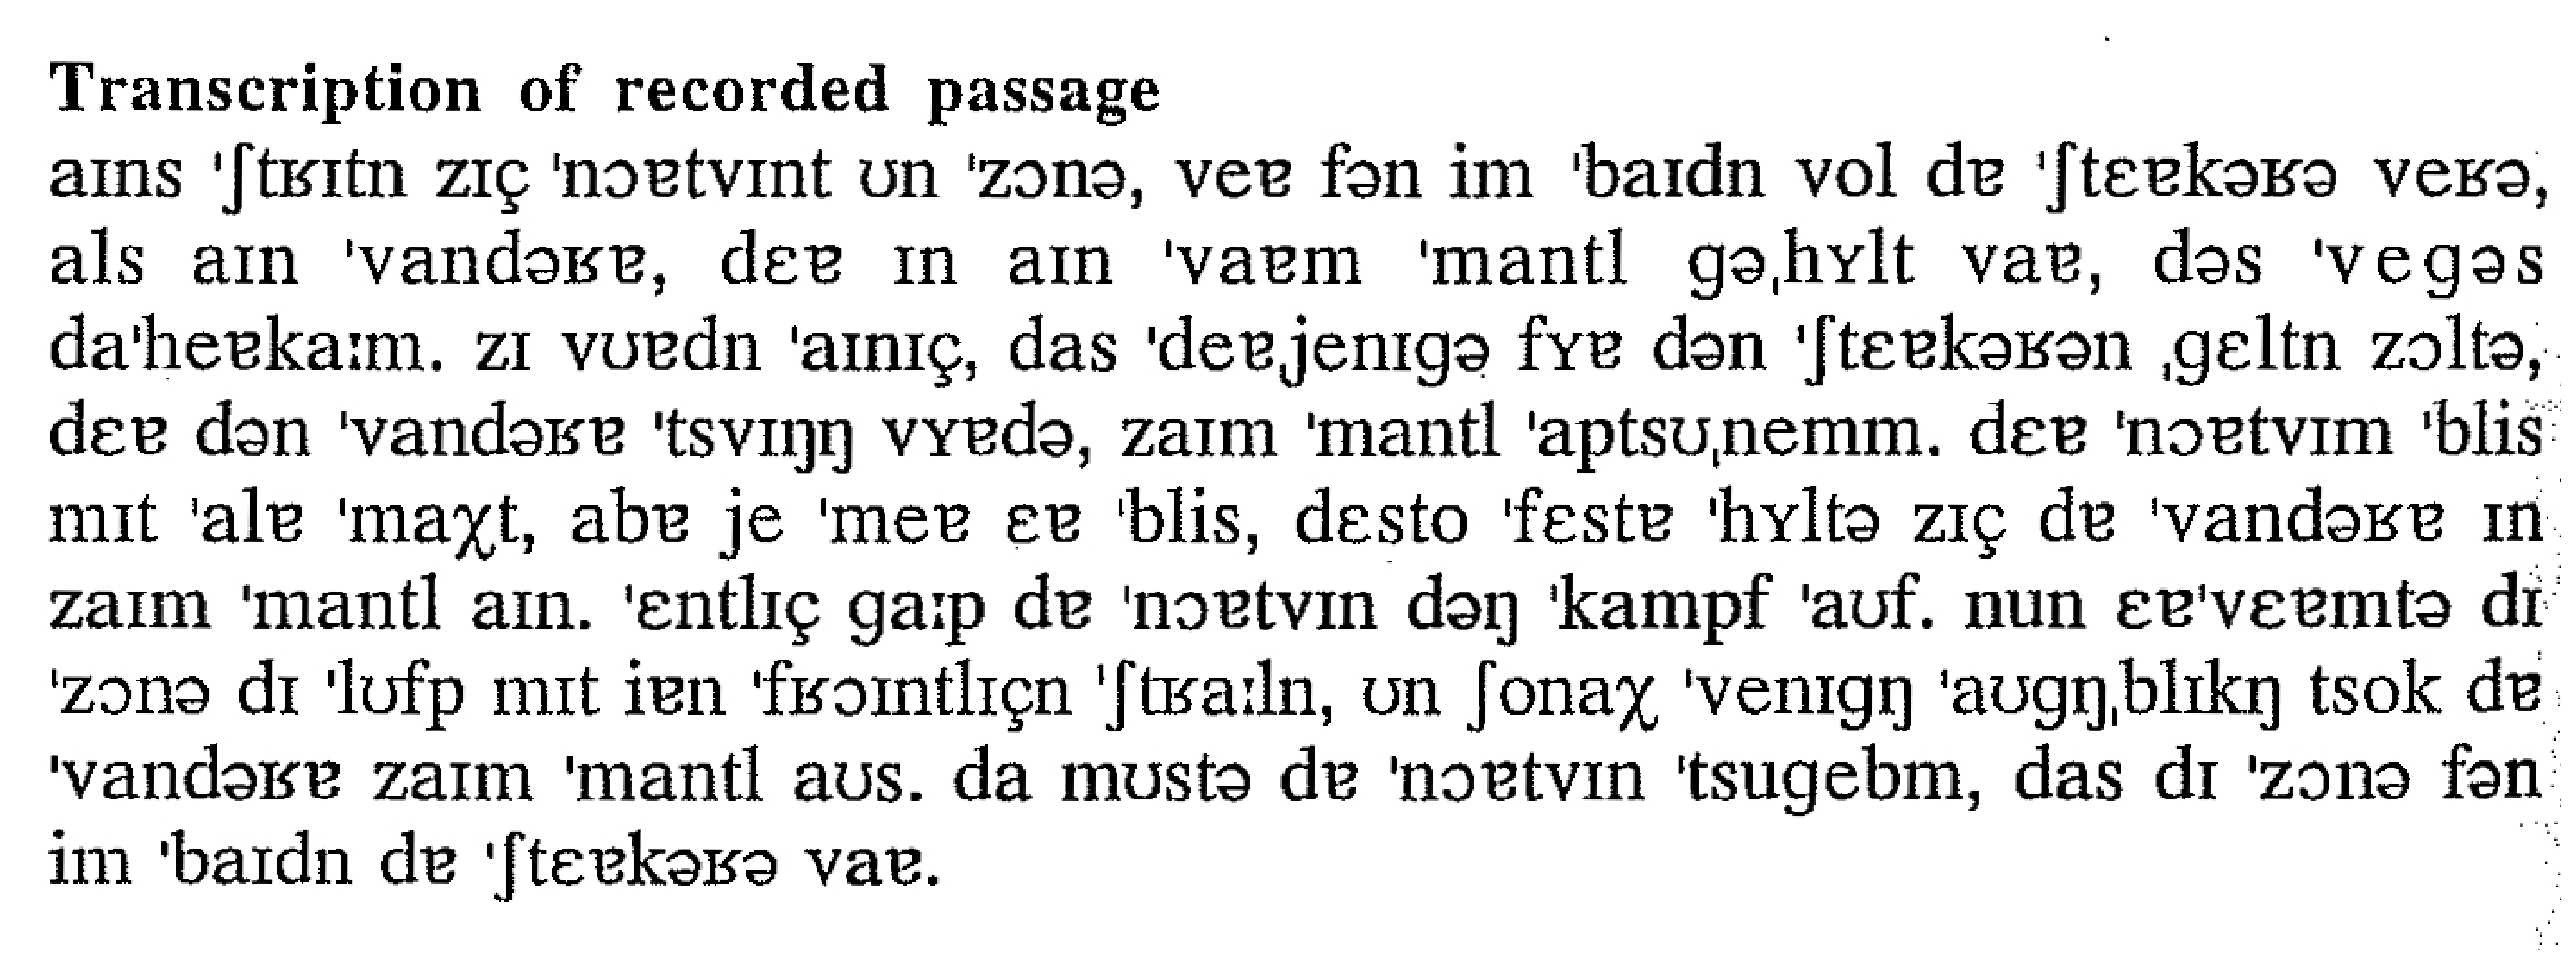
\includegraphics[scale=0.22]{material/04einststrittentranspompino}		
	%	\end{figure}


	\item \href{run:material/04einststrittenaudio/narrative_complete.mp3}{\textbf{SOUND}}
\end{itemize}


\end{frame}


%%%%%%%%%%%%%%%%%%%%%%%%%%%%%
\iftoggle{ue-loesung}{
	%%%%%%%%%%%%%%%%%%%%%%%%%%%%%%%%%%
%% UE 6 - 02 Phonetik
%%%%%%%%%%%%%%%%%%%%%%%%%%%%%%%%%%

\begin{frame}
\frametitle{Lösung: Text in IPA lesen}

\begin{itemize}
	\item {\footnotesize \textipa{aIns 'StKItn zI\c{c} \textprimstress nO5tvInt Un \textprimstress zOn@, v@5 f@n im \textprimstress baIdn vol d5 \textprimstress StE5k@K@ veK@, als aIn \textprimstress vand@K5, dE5 In aIn \textprimstress va5m \textprimstress mantl g@\textsecstress hylt va5, d@s \textprimstress veg@s da\textprimstress he5ka:m. zI vU5dn \textprimstress aInI\c{c}, das \textprimstress de5jenIg@ fy5 d@n \textprimstress StE5k@K@n \textsecstress gEltn zOlt@, dE5 d@n \textprimstress vand@K5 \textprimstress {tsvI\ng \ng}  {vy5d@}, zaIm \textprimstress mantl \textprimstress aptsU\textsecstress nemm. dE5 \textprimstress nO5tvIm \textprimstress blis mIt \textprimstress al5 \textprimstress maXt, ab5 je \textprimstress me5 E5 \textprimstress blis, dEsto \textprimstress fEst5 \textprimstress hylt@ zI\c{c} d5 \textprimstress vand@K5 In zaIm \textprimstress mantl aIn. \textprimstress EntlI\c{c} ga:p d5 \textprimstress nO5tvIn {d@\ng} \textprimstress kampf \textprimstress aUf. nun E5\textprimstress vE5mt@ dI \textprimstress zOn@ dI \textprimstress lUfp mIt i5n \textprimstress fKOIntlI\c{c}n \textprimstress StKa:ln, Un SonaX {\textprimstress venIg\ng} {\textprimstress aUg\ng \textsecstress blIk\ng} tsok d5 \textprimstress vand@K5 zaIm \textprimstress mantl aUs. da mUst@ d5 \textprimstress nO5tvIn \textprimstress tsugebm, das dI \textprimstress zOn@ f@n im \textprimstress baIdn d5 \textprimstress StE5k@K@ va5.}}
	
	\item \textcolor{red}{\footnotesize Einst stritten sich Nordwind und Sonne, wer von ihnen beiden wohl der Stärkere wäre, als ein Wanderer, der in einen warmen Mantel gehüllt war, des Weges daherkam. Sie wurden einig, dass derjenige für den Stärkeren gelten sollte, der den Wanderer zwingen würde, seinen Mantel abzunehmen. Der Nordwind blies mit aller Macht, aber je mehr er blies, desto fester hüllte sich der Wanderer in seinen Mantel ein. Endlich gab der Nordwind den Kampf auf. Nun erwärmte die Sonne die Luft mit ihrem freundlichen Strahlen, und schon nach wenigen Augenblicken zog der Wanderer seinen Mantel aus. Da musste der Nordwind zugeben, dass die Sonne von ihnen beiden der Stärkere war.}
	
	\hfill	(\citealp{Pompino95a}; \citealp[88--89]{Kohler99a})
	
\end{itemize}

\end{frame}


}
%%%%%%%%%%%%%%%%%%%%%%%%%%%%%


%%%%%%%%%%%%%%%%%%%%%%%%%%%%%%%%%%%
\subsection{Hausaufgabe}
%%%%%%%%%%%%%%%%%%%%%%%%%%%%%%%%%%%

%% MyP: Contents
\iftoggle{sectoc}{
	\frame{
		%\begin{multicols}{2}
		\frametitle{~}
		\tableofcontents[currentsubsection,subsubsectionstyle=hide]
		%\end{multicols}
	}
}

%%%%%%%%%%%%%%%%%%%%%%%%%%%%%%%%%%%%%%%%%%%%%%%%%%%%%%%

\begin{frame}
\frametitle{Hausaufgabe}

\begin{itemize}
	\item[1.] Transkribieren Sie folgende Wörter des Deutschen mit dem IPA:

	\begin{exe}
		\ex \label{ex:02HA1}
		\begin{xlist}
			\ex arbeiten
			\ex Giebel
			\ex sagen
			\ex fröhlich
			\ex Enge
			\ex Dampfschiff
		\end{xlist}
	\end{exe}

\end{itemize}

\end{frame}	


%%%%%%%%%%%%%%%%%%%%%%%%%%%%%%%%%%%
\begin{frame}
\frametitle{Hausaufgabe}

\begin{itemize}
	\item[2.] {Schreiben Sie für die folgenden Lautbeschreibungen das passende IPA-Symbol auf:}

 \begin{exe}
	 \ex \label{ex:02HA2}
 	\begin{xlist}
		\ex bilabialer stimmloser Plosiv
		\ex hoher vorderer ungerundeter gespannter Vokal
		\ex velarer dorsaler stimmloser Frikativ
		\ex  glottaler stimmloser Plosiv
		\ex  halbhoher fast vorderer ungerundeter ungespannter Vokal
		\ex  postalveolarer stimmhafter Frikativ
		\ex  halbtiefer zentraler ungerundeter Vokal
		\ex  obermittelhoher hinterer gerundeter gespannter Vokal
		\ex  alveolare koronale stimmlose Affrikate
		\ex  mittlerer zentraler ungerundeter Vokal
	\end{xlist}
\end{exe}
\end{itemize}

\end{frame}


%%%%%%%%%%%%%%%%%%%%%%%%%%%%%%%%%%
\begin{frame}
\frametitle{Hausaufgabe}

\begin{itemize}
	\item[3.] {Beschreiben Sie folgende Laute des Deutschen mit relevanten phonetischen Merkmalen:}
	
	\begin{exe}
		\ex \label{ex:02HA3}
		\begin{xlist}
			\ex \textipa{[y]}
			\ex \textipa{[x]}
			\ex \textipa{[\o]}
			\ex \textipa{[Z]}
			\ex \textipa{[t]}
			\ex \textipa{[E]}
			\ex \textipa{[m]}
			\ex \textipa{[O]}
		\end{xlist}
	\end{exe}

\end{itemize}

\end{frame}


%%%%%%%%%%%%%%%%%%%%%%%%%%%%%%%%
\begin{frame}{\textipa{[ S l U s ]}}

\begin{itemize}
	\item \textbf{VIDEO:} \href{run:material/04vocalcordssinging.mp4}{Vocal Chords}
\end{itemize}

\end{frame}


%%%%%%%%%%%%%%%%%%%%%%%%%%%%%
\iftoggle{ha-loesung}{
	%%%%%%%%%%%%%%%%%%%%%%%%%%%%%%%%%%
%% HA 1 - 02 Phonetik
%%%%%%%%%%%%%%%%%%%%%%%%%%%%%%%%%%

\begin{frame}
\frametitle{Hausaufgabe -- Lösung}

\begin{itemize}
	\item[1.] {Transkribieren Sie folgende Wörter des Deutschen mit dem IPA:}

		\begin{exe}
		\exr{ex:02HA1}
		\settowidth\jamwidth{XXXXXXXXXXXXXXXXXXXXXXXXXXXXXXXX} 
		\begin{xlist}
			\ex arbeiten\jambox{\only<2->{\textcolor{red}{
						\textipa{['PaK.b\texttoptiebar{aI}.t@n], ['Pa\;R.b\texttoptiebar{aI}.t@n], ['P\texttoptiebar{a5}.b\texttoptiebar{aI}.t@n]}
					}}}
			\ex Giebel\jambox{\only<3->{\textcolor{red}{
						\textipa{['gi:.b@l]}
					}}}
			\ex sagen\jambox{\only<4->{\textcolor{red}{
						\textipa{['za:.g@n]}
					}}}
			\ex fröhlich\jambox{\only<5->{\textcolor{red}{
						\textipa{['fr\o:.lI\c{c}]}
					}}}
			\ex Enge\jambox{\only<6->{\textcolor{red}{
						\textipa{['PE\.N@]}
					}}}
			\ex Dampfschiff\jambox{\only<7->{\textcolor{red}{
						\textipa{['dam\texttoptiebar{pf}.SIf]}
					}}}
		\end{xlist}
	\end{exe}

\end{itemize}

\end{frame}	


%%%%%%%%%%%%%%%%%%%%%%%%%%%%%%%%%%%
\begin{frame}
\frametitle{Hausaufgabe -- Lösung}

\begin{itemize}
	\item[2.] {Schreiben Sie für die folgenden Lautbeschreibungen das passende IPA-Symbol auf:}
	
	\begin{exe}
		\exr{ex:02HA2} 
		\settowidth\jamwidth{XXXXXX} 
		\begin{xlist}
			\ex bilabialer stimmloser Plosiv\jambox{\only<2->{\textcolor{red}{
						\textipa{[p]}
					}}}
			\ex hoher vorderer ungerundeter gespannter Vokal\jambox{\only<3->{\textcolor{red}{
					\textipa{[i:]}
				}}}
			\ex velarer dorsaler stimmloser Frikativ\jambox{\only<4->{\textcolor{red}{
						\textipa{[x]}
			}}}
			\ex glottaler stimmloser Plosiv\jambox{\only<5->{\textcolor{red}{
						\textipa{[P]}
			}}}
			\ex halbhoher fast vorderer ungerundeter ungespannter Vokal\jambox{\only<6->{\textcolor{red}{
					\textipa{[I]}
				}}}
			\ex postalveolarer stimmhafter Frikativ\jambox{\only<7->{\textcolor{red}{
						\textipa{[Z]}
					}}}
			\ex halbtiefer zentraler ungerundeter Vokal\jambox{\only<8->{\textcolor{red}{
						\textipa{[5]}
					}}}
			\ex obermittelhoher hinterer gerundeter gespannter Vokal\jambox{\only<9->{\textcolor{red}{
						\textipa{[o:]}
					}}}
			\ex alveolare koronale stimmlose Affrikate\jambox{\only<10->{\textcolor{red}{
						\textipa{[\texttoptiebar{ts}]}
			}}}
			\ex mittlerer zentraler ungerundeter Vokal\jambox{\only<11->{\textcolor{red}{
						\textipa{[@]}
			}}}
		\end{xlist}
	\end{exe}
	
\end{itemize}

\end{frame}


%%%%%%%%%%%%%%%%%%%%%%%%%%%%%%%%%%
\begin{frame}
\frametitle{Hausaufgabe -- Lösung}

\begin{itemize}
	\item[3.] {Beschreiben Sie folgende Laute des Deutschen mit relevanten phonetischen Merkmalen:}
	
	\begin{exe}
		\exr{ex:02HA3}
		\settowidth\jamwidth{XXXXXXXXXXXXXXXXXXXXXXXXXXXXXXXXXXXXXX}
		\begin{xlist}
			\ex \textipa{[y:]}\jambox{\only<2->{\textcolor{red}{
						hoher vorderer gerundeter gespannter Vokal
					}}}
			\ex \textipa{[x]}\jambox{\only<3->{\textcolor{red}{
						velarer dorsaler stimmloser Frikativ
					}}}
			\ex \textipa{[\o:]}\jambox{\only<4->{\textcolor{red}{
						obermittelhoher hinterer gerundeter gespannter Vokal
					}}}
			\ex \textipa{[Z]}\jambox{\only<5->{\textcolor{red}{
						postalveolarer koronaler stimmhafter Frikativ
					}}}
			\ex \textipa{[t]}\jambox{\only<6->{\textcolor{red}{
						alveolarer koronaler stimmloser Plosiv
					}}}
			\ex \textipa{[E]}\jambox{\only<7->{\textcolor{red}{
						untermittelhoher vorderer ungerundeter ungespannter Vokal
					}}}
			\ex \textipa{[m]}\jambox{\only<8->{\textcolor{red}{
						bilabialer stimmhafter Nasal
					}}}
			\ex \textipa{[O]}\jambox{\only<9->{\textcolor{red}{
						untermittelhoher hinterer gerundeter ungespannter Vokal
					}}}
		\end{xlist}
	\end{exe}
	
\end{itemize}

\end{frame}


}
%%%%%%%%%%%%%%%%%%%%%%%%%%%%%


%%%%%%%%%%%%%%%%%%%%%%%%%%%%%%%%%%%
%%%%%%%%%%%%%%%%%%%%%%%%%%%%%%%%%%%
\subsection*{Abbildungen}
%%%%%%%%%%%%%%%%%%%%%%%%%%%%%%%%%%%

\begin{frame}[allowframebreaks]{Abbildungen}
	\footnotesize
		
		\begin{itemize}
			\item ABBILDUNG -- \gqq{Rousselots Apparat zur Aufzeichnung der Sprache} (Zugriff: 09.12.16): \url{https://de.wikipedia.org/wiki/Jean-Pierre\_Rousselot\#/media/File:Rousselots\_Apparat\_zur\_Aufzeichnung\_der\_Sprache.jpg}

			\item ABBILDUNG -- \gqq{Spektrogramm \gq{Pronouncing}} (Autor: Rjanag, Zugriff: 20.12.16): \url{https://upload.wikimedia.org/wikipedia/commons/3/30/Pronouncing.PNG?uselang=de}

			\item ABBILDUNG -- Abbildung \gqq{IPA vowel chart} (CC BY-SA 3.0, Zugriff: 09.12.16): \url{https://en.wikipedia.org/w/index.php?curid=3368128}

			\item ABBILDUNG -- \gqq{Sagittalschnitt} (CC BY-SA 3.0, Zugriff: 09.12.16): \url{https://commons.wikimedia.org/w/index.php?curid=2615572}
		\end{itemize}	
	
\end{frame}


%%%%%%%%%%%%%%%%%%%%%%%%%%%%%%%%%%%
%%%%%%%%%%%%%%%%%%%%%%%%%%%%%%%%%%%
\subsection*{Elektronische Quellen}
%%%%%%%%%%%%%%%%%%%%%%%%%%%%%%%%%%%

\begin{frame}[allowframebreaks]{Elektronische Quellen}

	\footnotesize
	
	\begin{itemize}
	
		\item VIDEO -- \gqq{Spoken Pirahã with subtitles} (Zugriff: 24.10.2013): \url{http://www.youtube.com/watch?v=SHv3-U9VPAs}

		\item LINK -- \gqq{Webseite der IPA} (Zugriff: 24.10.2013): \url{http://internationalphoneticassociation.org}

		\item LINK -- \gqq{Peter Ladefoged -- A Course in Phonetics} (Zugriff: 24.10.2013):
		\url{http://phonetics.ucla.edu/course/chapter1/chapter1.html}
		
		\item VIDEO -- \gqq{!Nama Clicks} (Zugriff: 24.10.2013): \url{http://www.youtube.com/watch?v=Ophrf64fxgA&list=PL6rcWnFnBuT7BEAex2IvI6l_bjLLycxaU}

		\item VIDEO -- \gqq{Anatomical Tutorial During Trans-Nasal Endoscopy} (Zugriff: 24.10.2012): \url{http://www.youtube.com/watch?v=wjRsa77u6OU}

		\item LINK -- \gqq{Interactive Sagittal Section} (Zugriff: 27.04.2016): \url{http://smu-facweb.smu.ca/~s0949176/sammy/}
		
		\item LINK -- \gqq{Interactive IPA chart} (Zugriff: 23.10.2019):
		\url{http://www.ipachart.com/}

		\item VIDEO -- \gqq{Vocal Chords up close while singing} (Zugriff: 24.10.2012): \url{http://www.youtube.com/watch?v=-XGds2GAvGQ}
		
		\item SOUND -- \gqq{Enge Transkription} (Zugriff: 22.11.2018):
		\url{https://www.internationalphoneticassociation.org/sites/default/files/handbookfiles/German.zip}
		
		\item VIDEO -- \gqq{Aspiration} (Zugriff: 27.11.2018)
		\url{https://www.youtube.com/watch?v=6PSdlctYBsw&index=62&list=PL6rcWnFnBuT7BEAex2IvI6l_bjLLycxaU&t=3s}
	\end{itemize}
	
\end{frame}

